\documentclass[12pt,a4paper,oneside]{report}
\usepackage[utf8]{inputenc}
\usepackage[T1]{fontenc}
\usepackage{mathptmx}
\usepackage[scaled=0.9]{helvet}
\usepackage{geometry}
\geometry{a4paper,left=1.5in,right=1in,top=1.2in,bottom=1.2in}
\usepackage{setspace}
\onehalfspacing
\usepackage{graphicx}
\graphicspath{{images/}}
\usepackage{amsmath,amssymb}
\usepackage{booktabs,array,multirow,longtable,tabularx}
\usepackage{caption}
\captionsetup{font=small,labelfont=bf,justification=centering}
\usepackage{subcaption}
\usepackage{xcolor}
\definecolor{isiblue}{RGB}{30,70,130}
\usepackage{float}
\newfloat{algorithm}{tbp}{loa}
\floatname{algorithm}{Algorithm}
\newcommand{\listofalgorithms}{\listof{algorithm}{List of Algorithms}}
\newenvironment{algbody}{%
  \par\vspace{2pt}\hrule\vspace{3pt}\small\raggedright
  \setlength{\parindent}{0pt}\setlength{\parskip}{1.5pt}}{%
  \par\vspace{3pt}\hrule\vspace{2pt}}
\newcommand{\albf}[1]{\textbf{#1}}
\newcommand{\aln}[1]{\makebox[1.7em][r]{#1}\hspace{0.6em}}
\newcommand{\alin}{\hspace*{1.4em}}
\newcommand{\alinn}{\hspace*{2.8em}}
\usepackage{enumitem}
\usepackage{microtype}
\usepackage{fancyhdr}
\setlength{\headheight}{14pt}
\usepackage[hidelinks]{hyperref}
\hypersetup{colorlinks=true,linkcolor=black,citecolor=isiblue,urlcolor=isiblue}
\pagestyle{fancy}
\fancyhf{}
\renewcommand{\headrulewidth}{0.4pt}
\fancyhead[L]{\small\leftmark}
\fancyfoot[C]{\thepage}
\renewcommand{\chaptermark}[1]{\markboth{\chaptername\ \thechapter.\ #1}{}}
\newcommand{\zvec}{\mathbf{z}}
\newcommand{\hvec}{\mathbf{h}}
\newcommand{\Dmean}{D_{\mathrm{mean}}}
\newcommand{\Vlast}{V_{\mathrm{last}}}
\newcommand{\Hmean}{H_{\mathrm{mean}}}
\begin{document}
\begin{titlepage}
\centering
\vspace*{0.4cm}
{\large Indian Statistical Institute}\\[0.2cm]
{\small Kolkata 700108, India}\\[1.6cm]
{\LARGE\bfseries Hallucination Detection in Large\\[0.2cm]
Language Models Using Internal\\[0.2cm] Representations\par}
\vspace{1.4cm}
{\normalsize DISSERTATION SUBMITTED IN PARTIAL FULFILLMENT OF THE\\
REQUIREMENTS FOR THE DEGREE OF\par}
\vspace{0.6cm}
{\large\bfseries Master of Technology\par}
\vspace{0.2cm}
{\normalsize in\par}
\vspace{0.2cm}
{\large Computer Science (with specialization in Data Science)\par}
\vspace{1.0cm}
{\normalsize by\par}
\vspace{0.3cm}
{\large\bfseries Chinmoy Sahoo\par}
{\normalsize [\,Roll No: CS2412\,]\par}
\vspace{1.0cm}
{\normalsize under the supervision of\par}
\vspace{0.3cm}
{\large\bfseries Prof.\ Ujjwal Bhattacharya\par}
{\normalsize Professor\\
Computer Vision and Pattern Recognition Unit\\
Indian Statistical Institute\\
Kolkata 700108, India\par}
\vfill
{\normalsize June 2026\par}
\end{titlepage}
\pagenumbering{roman}
\setcounter{page}{1}
\chapter*{Certificate}
\addcontentsline{toc}{chapter}{Certificate}
\thispagestyle{plain}
\vspace{0.5cm}
This is to certify that the dissertation entitled \textbf{``Hallucination Detection
in Large Language Models Using Internal Representations''} submitted by
\textbf{Chinmoy Sahoo} (Roll No: CS2412) to the Indian Statistical Institute,
Kolkata, in partial fulfilment of the requirements for the award of the degree of
\textbf{Master of Technology in Computer Science (with specialization in Data
Science)} is a bona fide record of work carried out by him under my supervision and
guidance. The dissertation has fulfilled all the requirements as per the regulations
of this institute and, in my opinion, has reached the standard needed for submission.
\vspace{2.5cm}
\noindent
\begin{flushright}
\textbf{Prof.\ Ujjwal Bhattacharya}\\
Professor,\\
Computer Vision and Pattern Recognition Unit,\\
Indian Statistical Institute,\\
Kolkata 700108, India.
\end{flushright}
\chapter*{Declaration}
\addcontentsline{toc}{chapter}{Declaration}
\thispagestyle{plain}
\vspace{0.5cm}
I hereby declare that the work presented in this dissertation, entitled
\textbf{``Hallucination Detection in Large Language Models Using Internal
Representations''}, is the result of my own investigation carried out under the
supervision of Prof.\ Ujjwal Bhattacharya at the Computer Vision and Pattern
Recognition Unit, Indian Statistical Institute, Kolkata. All external sources of
information, ideas and figures have been duly acknowledged and cited. To the best of
my knowledge, this work has not been submitted, in whole or in part, for any other
degree or diploma.
\vspace{2.5cm}
\noindent
\begin{flushright}
\textbf{Chinmoy Sahoo}\\
Roll No: CS2412\\
Indian Statistical Institute,\\
Kolkata 700108, India.
\end{flushright}
\clearpage
\thispagestyle{plain}
\vspace*{6cm}
\begin{center}
\textit{To my parents and my teachers,\\[0.3cm]
for their patience and their faith in slow, careful work.}
\end{center}
\chapter*{Acknowledgements}
\addcontentsline{toc}{chapter}{Acknowledgements}
\thispagestyle{plain}
I owe my deepest gratitude to my supervisor, Prof.\ Ujjwal Bhattacharya, of the
Computer Vision and Pattern Recognition Unit at the Indian Statistical Institute,
Kolkata. His steady guidance, his insistence on careful claims over comfortable ones,
and his encouragement to keep the experimental scope honest shaped this dissertation
at every stage.
I am thankful to the faculty and research staff of the Institute for building an
environment in which ideas can be tested rather than merely asserted, and for the
computational guidance that made a free-tier study of this kind feasible. I thank my
fellow students for many useful discussions on language models, evaluation, and the
practical difficulties of running large models on modest hardware.
Finally, I thank my family for their unwavering support throughout this work.
\vspace{1cm}
\begin{flushright}
\textbf{Chinmoy Sahoo}\\
Indian Statistical Institute,\\
Kolkata 700108, India.
\end{flushright}
% ---------------- ABSTRACT ----------------
\chapter*{Abstract}
\addcontentsline{toc}{chapter}{Abstract}

Large language models produce fluent text that is sometimes confidently wrong. This
failure, commonly called \emph{hallucination}, is now the dominant practical obstacle
to deploying such models where correctness matters. A promising line of detectors
reads the model's own internal activations as it generates, and learns to tell
truthful continuations from fabricated ones without any external retrieval and without
sampling the model many times. These detectors are attractive because they add almost
no cost at inference time, but the published results are scattered across different
models, datasets, and hardware budgets, which makes it hard to know how much each
ingredient actually contributes.

This dissertation studies internal-state hallucination detection under a single,
reproducible protocol that runs entirely on free cloud hardware. We adopt the
label-free data-generation idea of the MIND framework, in which a model continues a
truncated encyclopedia article and the continuation is automatically labelled by
whether the model recovers the original entity. On top of the canonical last-token,
last-layer hidden state used by that framework, we add three inexpensive signals
computed from the same forward pass: how much the representation shifts from one layer
to the next, how much it varies across layers, and how uncertain the model is while
generating. We then compare this augmented detector against a wider set of literature
features and against four established baselines, together with two simple reference
methods, across as many as ten question-answering, summarisation, and dialogue
benchmarks.

We report only the results that our saved measurement files support, and we separate
\emph{in-distribution} detection (held-out encyclopedia text) from \emph{cross-task
transfer} (the question-answering and dialogue benchmarks), because the two regimes
behave very differently. On the fully measured six-billion-parameter model, the
richest feature configurations are competitive with the strongest baseline but do not
overtake it, and a single benchmark heavily influences the averages; on a second model
of comparable size an earlier extended run favoured one of the proposed feature
configurations. The honest summary is that the value of these internal-state features
is real but \emph{model dependent}, and that cross-task transfer remains the hard part.
The contribution of this work is therefore not a new state-of-the-art detector but a
careful, free-tier-reproducible comparison of internal-state features across several
open models, with an explicit account of what is measured, what is still pending, and
where the method's limits lie.

\vspace{0.4cm}
\noindent\textbf{Keywords:} hallucination detection, large language models, internal
representations, hidden states, probing classifiers, model calibration, reproducible
evaluation.

\clearpage
\tableofcontents
\clearpage
\addcontentsline{toc}{chapter}{List of Figures}
\listoffigures
\clearpage
\addcontentsline{toc}{chapter}{List of Tables}
\listoftables
\clearpage
\addcontentsline{toc}{chapter}{List of Algorithms}
\listofalgorithms
% ---------------- ABBREVIATIONS ----------------
\clearpage
\chapter*{List of Abbreviations}
\addcontentsline{toc}{chapter}{List of Abbreviations}
\markboth{List of Abbreviations}{}

\begin{center}
\renewcommand{\arraystretch}{1.25}
\begin{tabular}{p{2.6cm} p{10.5cm}}
\toprule
\textbf{Abbrev.} & \textbf{Expansion} \\
\midrule
LLM     & Large Language Model \\
MIND    & The internal-state hallucination-detection framework of Su et al.~(2024) that this work extends; used as a proper name \\
MLP     & Multi-Layer Perceptron \\
AUROC   & Area Under the Receiver-Operating-Characteristic curve \\
ROC     & Receiver Operating Characteristic \\
ECE     & Expected Calibration Error \\
QA      & Question Answering \\
NLI     & Natural Language Inference \\
JSD     & Jensen--Shannon Divergence \\
SOTA    & State Of The Art \\
BLEURT  & Bilingual Evaluation Understudy with Representations from Transformers (a learned text-similarity metric) \\
VRAM    & Video Random-Access Memory (GPU memory) \\
bf16    & The bfloat16 16-bit floating-point number format \\
HF      & Hugging Face (model and dataset hub) \\
NLL     & Negative Log-Likelihood \\
SVD     & Singular Value Decomposition \\
\bottomrule
\end{tabular}
\end{center}

\noindent\small Each abbreviation is also defined in words at its first use in the
chapter where it first appears.

\clearpage
\pagenumbering{arabic}
\setcounter{page}{1}
% =====================================================================
\chapter{Introduction}
\label{ch:intro}
% =====================================================================

\section{Motivation}

A large language model, hereafter abbreviated LLM, is a neural network trained to
predict the next token in a sequence of text. Once trained on enough data, such a model
can answer questions, summarise documents, and hold a conversation. The same property
that makes these systems useful also makes them dangerous in a specific way: they are
optimised to produce text that \emph{looks} right, not text that \emph{is} right. As a
result, an LLM will sometimes state a wrong fact with the same fluency and confidence
that it uses for a correct one. This behaviour is widely called \emph{hallucination},
and a now-standard survey of the topic describes it as the generation of content that
is fluent and plausible yet unfaithful to the source or to the world~\cite{ji2023survey}.

Hallucination is not a rare glitch. It is a structural consequence of how these models
are built, and it appears across every task to which LLMs are applied. When a model
invents a citation, misstates a medical dosage, or confidently answers a question whose
premise is false, the cost is borne by whoever trusted the answer. As LLMs move from
demonstrations into tools that professionals rely on, the ability to attach a warning
to an unreliable answer becomes as important as the answer itself. The problem this
dissertation addresses is therefore not how to stop a model from hallucinating, but how
to \emph{detect}, cheaply and in real time, when it probably has.

Several families of detectors exist, and we review them in detail in
Chapter~\ref{ch:related}. One popular family samples the model many times and checks
whether the answers agree, on the intuition that fabricated content is unstable while
real knowledge is consistent; the best-known method of this kind is
SelfCheckGPT~\cite{manakul2023selfcheckgpt}. This approach works without any access to
the model's internals, but it is expensive: it requires many full generations for every
single answer it checks. A second family takes the opposite view. It assumes we can open
the model up and read the hidden activations it produces while generating, and it learns
a small classifier that maps those activations to a hallucination probability. The
appeal is cost. Because the activations are already computed during normal generation,
reading them adds almost nothing to the running time. Figure~\ref{fig:latency}
illustrates the gap that motivates this entire line of work: a sampling-based check can
cost hundreds of times more per response than an internal-state probe.

\begin{figure}[t]
\centering
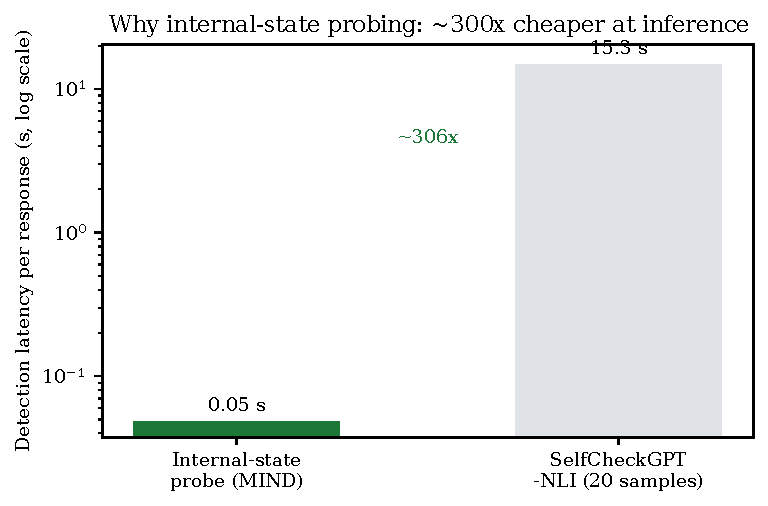
\includegraphics[width=0.62\textwidth]{images/ch01_intro/ch01_1_latency.pdf}
\caption{The practical case for internal-state probing. A consistency check that draws
roughly twenty extra samples per response costs orders of magnitude more time than a
classifier that reads activations the model has already produced. Latencies are
indicative figures from the internal-state detection literature, plotted on a
logarithmic scale.}
\label{fig:latency}
\end{figure}

The internal-state family began with the observation that a model's hidden layers seem
to ``know'' when the model is producing a falsehood, even when its surface output gives
no hint~\cite{azaria2023saplma}. Building on this, the MIND framework showed that one
can generate the training labels automatically, rather than by hand, and still train an
effective and fast detector~\cite{su2024mind}; here MIND refers to the model
internal-state-based detection method of Su et al., which we adopt as our starting
point. Later work pushed the idea further, either by removing the need for any labels at
all~\cite{du2024haloscope} or by fusing signals from every layer of the
network~\cite{dasgupta2025hallushift}. These methods are promising, but they have been
reported under inconsistent conditions, and crucially most of them were demonstrated on
large models running on research-grade hardware. Whether the same signals survive on
the smaller open models that a student or a small team can actually run, and how the
many proposed features compare on equal footing, is the gap this dissertation sets out
to fill.

\section{Problem Statement}

The central question of this work can be stated plainly:

\begin{quote}
\emph{Given an open-weights language model running on free, memory-limited hardware, how
reliably can we detect hallucinations by reading internal representations from a single
forward pass, and which internal-state signals are worth their cost?}
\end{quote}

This question has three parts that are easy to conflate and that we deliberately keep
separate throughout the dissertation. The first part is the \emph{detection signal}:
which quantities, computed from the hidden states and the output distribution, carry
information about whether the current generation is faithful. The second part is the
\emph{evaluation regime}: a detector trained on one kind of text (here, automatically
labelled encyclopedia continuations) may work well on similar text but transfer poorly
to question answering, summarisation, or dialogue. Reporting a single headline number
hides this distinction, so we always separate held-out in-distribution performance from
cross-task transfer. The third part is the \emph{compute budget}: a method that needs
multiple samples, a singular-value decomposition, or a large auxiliary model may be
accurate but impractical on the hardware we target. A useful detector has to be honest
on all three axes at once.

A complication specific to this work is that a closely related study exists at the same
institute, conducted independently in a different research group, which targets the same
benchmark suite. To keep the present contribution clearly its own, the design of our
detector deliberately differs from that prior study at the level of features and
classifier; this separation is explained where the relevant method is introduced in
Chapter~\ref{ch:related} and respected throughout.

\section{Research Objectives}

The objectives of the dissertation are the following.

\begin{enumerate}[leftmargin=2.2em,itemsep=0.3em]
\item To re-implement the label-free, internal-state detection pipeline of the MIND
framework~\cite{su2024mind} so that it runs end to end on free cloud GPUs, and to verify
its correctness with a small diagnostic model before scaling up.

\item To design three inexpensive internal-state features --- layer-wise representation
drift, cross-layer variance, and predictive entropy --- that are computed from the same
forward pass as the existing canonical feature, and to define them in clean,
self-contained notation.

\item To assemble a single ablation that compares the canonical feature, the three new
features, a set of nine features drawn from the recent literature, and a further set of
exploratory features, under one fixed classifier and one fixed evaluation protocol.

\item To evaluate this ablation against four established baselines and two simple
reference methods across a multi-task benchmark suite spanning question answering,
summarisation, and dialogue, on several open models of different sizes.

\item To report the outcome honestly: to state which numbers are backed by saved
measurements, to keep in-distribution and transfer results apart, and to avoid any claim
of superiority that the measurements do not support.
\end{enumerate}

\section{Thesis Contributions}

The contributions of this dissertation are modest by design and are stated as such.

\textbf{A free-tier-reproducible comparison.} The primary contribution is a unified,
reproducible comparison of internal-state hallucination features across multiple open
LLMs, built to run within the memory and time limits of free cloud notebooks. Every
configuration shares the same automatically generated training data, the same
classifier, the same train/test split, and the same evaluation rows, so that
differences in measured performance can be attributed to the features rather than to
incidental differences in setup.

\textbf{Three forward-pass features and a clean ablation.} We introduce three
additional internal-state signals on top of the canonical hidden state and place them
in an ablation alongside literature features and exploratory features. The ablation
isolates what each family of features adds, rather than reporting only a single combined
system.

\textbf{An honest, regime-separated account of the results.} We show that, on the model
for which we have a complete set of measurements, the richer feature configurations are
competitive with the strongest baseline but do not surpass it, and that a single
benchmark dominates the averages. We further show that cross-task transfer is markedly
harder than in-distribution detection. We treat these findings, including the ones that
are unflattering to the proposed features, as the result.

It is worth stating clearly what this dissertation does \emph{not} claim. It does not
claim a new state-of-the-art detector, it does not claim to beat any prior method on its
own benchmark, and it does not present results for experiments whose measurement files
are not yet complete. Where an experiment is still running, it is marked as pending.

\section{Thesis Organization}

The remainder of the dissertation is organised as follows.

\textbf{Chapter~\ref{ch:background}} provides the background needed to read the rest of
the work: how transformer language models produce hidden states, what a hallucination is
in precise terms, and how detection is measured.

\textbf{Chapter~\ref{ch:related}} surveys the literature on hallucination detection,
organising it into four families and positioning the present work within the
internal-state family. It is here that the related institute study is cited once, as
adjacent prior work, with an explicit account of how our method differs.

\textbf{Chapter~\ref{ch:method}} presents the methodology: the automatic label
generation, the canonical feature and the three new internal-state features in full
notation, the wider feature families, the classifier, the baselines, and the
free-hardware implementation.

\textbf{Chapter~\ref{ch:results}} reports the experiments. It presents the verified
results, separates in-distribution from transfer performance, discusses the strengths
and weaknesses of the proposed features, and marks the experiments that are still in
progress.

\textbf{Chapter~\ref{ch:conclusion}} summarises what was found, states the limitations
without softening them, and lays out concrete next steps.

% =====================================================================
\chapter{Background}
\label{ch:background}
% =====================================================================

This chapter sets out the minimum background needed to follow the rest of the
dissertation. It explains how a transformer language model turns text into internal
vectors, states precisely what we mean by a hallucination, frames detection as a
classification problem, and defines the metrics used to score a detector. A reader
already familiar with transformer internals and detection metrics can skim this chapter
and move on to Chapter~\ref{ch:related}.

\section{Transformer language models and their hidden states}

Modern language models are built from the transformer architecture~\cite{vaswani2017attention}.
The input text is first broken into \emph{tokens} --- sub-word units --- and each token
is mapped to a vector. These vectors then pass through a stack of identical layers. Each
layer mixes information between token positions using a mechanism called
\emph{self-attention}, and then transforms each position independently through a small
feed-forward network. The output of every layer is, again, one vector per token. We
write $\zvec_\ell^{(t)}$ for the vector that layer $\ell$ produces at token position
$t$, and we call it the \emph{activation} or \emph{hidden state} at that layer and
position. A model with $L$ layers therefore produces a whole stack of activations
$\zvec_1^{(t)}, \zvec_2^{(t)}, \dots, \zvec_L^{(t)}$ for each position it processes.

After the final layer, the model multiplies the last activation by an output matrix to
obtain a score for every possible next token, and a softmax turns these scores into a
probability distribution $p_t(\cdot)$ over the vocabulary. The token with the highest
probability is usually emitted, the text grows by one token, and the process repeats.
Two facts about this picture matter for the rest of the dissertation. First, the entire
stack of activations is computed anyway during normal generation, so anything we derive
from it is essentially free. Second, the activations are high-dimensional --- a few
thousand numbers per token for the models we study --- and they are believed to encode
not only \emph{what} the model is saying but also something about \emph{how sure} and
\emph{how grounded} it is. The central bet of internal-state detection is that this
``something'' can be read out.

The dimensionality of a model's hidden state, written $d$, and its number of layers $L$
vary with model size. The models used in this dissertation range from a small diagnostic
model with a few hundred million parameters up to seven-billion-parameter models; the
six-billion-parameter model that anchors our results has $d = 4096$ and $L = 28$ layers.
These sizes are reported in full in Chapter~\ref{ch:method}.

\section{What counts as a hallucination}

The word ``hallucination'' covers more than one phenomenon, and being careful about the
distinctions avoids confusion later. Following the standard
survey~\cite{ji2023survey}, we separate two axes.

The first axis is \emph{intrinsic} versus \emph{extrinsic}. An intrinsic hallucination
contradicts the material the model was given: a summary that reverses what an article
actually said is intrinsic. An extrinsic hallucination adds content that cannot be
checked against the given material --- it may happen to be true or false in the world,
but it is unsupported by the input.

The second axis is \emph{faithfulness} versus \emph{factuality}. Faithfulness asks
whether the output is consistent with the prompt or source document; factuality asks
whether it is consistent with the real world. A model can be faithful but not factual
(it accurately reflects a flawed source) or factual but not faithful (it states a true
fact the source never mentioned). Different benchmarks target different corners of this
space, which is one reason a detector that does well on one benchmark may do poorly on
another.

A third consideration is \emph{granularity}: a hallucination label can be attached to a
whole passage, to a sentence, or to an individual fact. Finer labels are more useful but
harder to obtain. The approach we build on produces labels automatically at the level of
a generated continuation, which sidesteps the cost of human annotation; the price is
that the labels are only as good as the automatic procedure that creates them, a point
we return to in Chapter~\ref{ch:method}.

Throughout the dissertation we use the operational definition adopted by the method we
extend: a hallucination is a coherent but factually incorrect span of generated text,
where ``incorrect'' is judged against an external reference such as an encyclopedia
article or a gold question--answer pair.

\section{Detection as a classification problem}

Once labels exist, detection becomes a supervised classification problem. For each
generated example we form a feature vector $\mathbf{x}$ from the model's internal state,
and we attach a binary label $y$, where $y=0$ marks a faithful generation and $y=1$
marks a hallucinated one. A classifier is then trained to estimate
$P(y = 1 \mid \mathbf{x})$. In this work the classifier is a multi-layer perceptron,
abbreviated MLP: a feed-forward neural network of several layers that maps the feature
vector to a probability. The detector's quality depends almost entirely on whether
$\mathbf{x}$ carries the right information, which is why the design of the features ---
the subject of Chapter~\ref{ch:method} --- is where the real work lies.

A subtle but important point is the difference between two evaluation regimes. If the
classifier is trained and tested on the same kind of text, we measure
\emph{in-distribution} detection. If it is trained on one kind of text (encyclopedia
continuations) and tested on another (question answering, summarisation, dialogue), we
measure \emph{transfer}. Transfer is the harder and more realistic setting, and as
Chapter~\ref{ch:results} shows, the two regimes can give very different numbers for the
same detector. We never average across them.

\section{How detection is measured}

Because a detector outputs a probability, it can be scored either as a ranking or as a
calibrated estimate. We use the following metrics, each defined here at first use.

\textbf{AUROC.} The area under the receiver-operating-characteristic curve, abbreviated
AUROC, measures how well the detector \emph{ranks} hallucinated examples above faithful
ones. It equals the probability that a randomly chosen hallucinated example receives a
higher score than a randomly chosen faithful one. A perfect detector scores $1.0$, and
a detector that guesses scores $0.5$. AUROC is the headline metric in most of the
internal-state literature because it does not depend on a particular decision threshold,
and it is the metric we use for cross-method comparison.

\textbf{Accuracy, precision, recall, F1.} These threshold-dependent metrics summarise
the confusion matrix once a cut-off is chosen. Accuracy is the fraction of correct
decisions; precision is the fraction of flagged examples that really were hallucinated;
recall is the fraction of true hallucinations that were flagged; and F1 is the harmonic
mean of precision and recall. They are useful but can be misleading when the two classes
are imbalanced or when the classifier collapses to predicting a single class, a failure
mode we observe at small data scales.

\textbf{Brier score and ECE.} A detector is well \emph{calibrated} if a stated
probability of, say, $0.8$ is right about $80\%$ of the time. The Brier score is the
mean squared difference between the predicted probability and the true label; the
expected calibration error, abbreviated ECE, bins predictions by confidence and measures
how far the average confidence in each bin is from the observed accuracy. Lower is better
for both. We report these where our measurement files contain them, because a calibrated
probability is more useful in practice than a bare yes/no verdict.

A final caution applies to all of these numbers. When a benchmark is small, a metric
estimated on it is noisy, and a single easy or hard dataset can dominate an average
computed over several benchmarks. We flag both effects explicitly when they occur in
Chapter~\ref{ch:results}, rather than letting a headline average paper over them.

% =====================================================================
\chapter{Related Work}
\label{ch:related}
% =====================================================================

This chapter reviews the literature on hallucination detection and locates the present
dissertation within it. We group the field into four families, sketched in
Figure~\ref{fig:taxonomy}, and devote the most attention to the internal-state family
that this work extends. The chapter closes by describing the benchmarks the area uses,
the open problems it has identified, and the specific slot this dissertation occupies.

\begin{figure}[t]
\centering
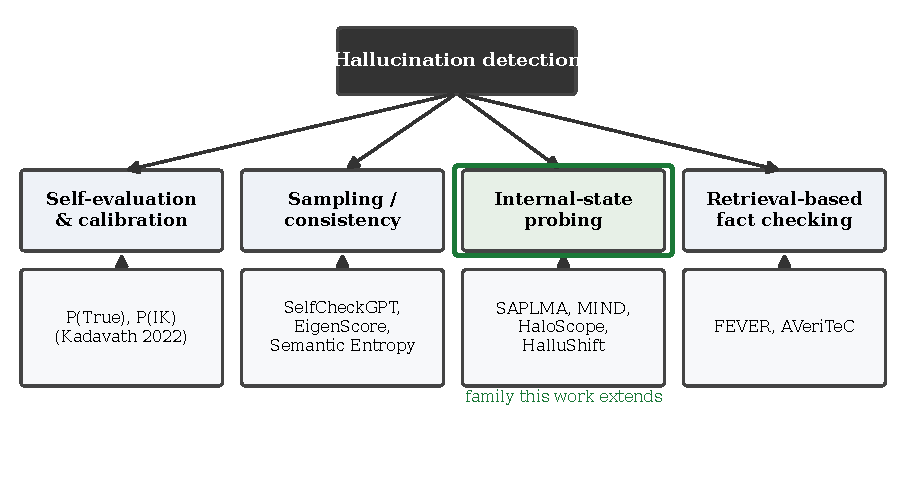
\includegraphics[width=0.96\textwidth]{images/ch03_related_work/ch03_1_taxonomy.pdf}
\caption{Four families of hallucination detection. This dissertation works in the
internal-state probing family (outlined), which reads a model's own activations and is
the cheapest to run at inference time.}
\label{fig:taxonomy}
\end{figure}

\section{Why surface-overlap metrics are not enough}

The earliest way to judge a generation was to compare it, word for word, against a
reference using overlap scores such as ROUGE or BLEU. These remain common as headline
numbers, but they measure surface similarity, not truth. The standard cautionary example
makes the point: the sentence ``Paris is the capital of Germany'' shares almost every
word with ``Paris is the capital of France'' and would earn a near-perfect overlap
score, despite being false. Surface form is a poor proxy for meaning, and a worse proxy
for factual correctness. The field has therefore moved to \emph{semantic} detectors that
do not rely on word overlap, and these fall into the four families below.

\section{Family I: self-evaluation and calibration}

The first idea is to ask the model to judge itself. The line begins with work showing
that large models are often reasonably \emph{calibrated}: the probability they assign to
an answer tracks how often that answer is correct~\cite{kadavath2022know}. Two probes
from that work are still influential. The first reads the probability the model assigns
to the token ``True'' after being asked to evaluate its own answer; the second trains a
small head to predict, from the question alone, whether the model is likely to answer
correctly. Both establish that a usable uncertainty signal exists inside the model, and
both are ancestors of the probing classifiers discussed later. Their limitation is that
self-evaluation tends to generalise only partially: a probe tuned on one task degrades
under distribution shift, a recurring theme that returns in our own transfer results.

\section{Family II: sampling and consistency}

A second family ignores the internals entirely and treats the model as a black box. The
idea is simple: generate an answer, then draw several more samples at a higher
temperature, and check whether they agree. Factual content tends to stay stable across
samples, while fabricated content tends to wobble. The canonical method,
SelfCheckGPT~\cite{manakul2023selfcheckgpt}, implements this consistency check at several
levels of abstraction, from word-overlap to a natural-language-inference model
(abbreviated NLI: a classifier that decides whether one sentence entails or contradicts
another). On a benchmark of generated biographies it detects non-factual sentences well
and needs no labels, no internals, and no retrieval --- only the ability to sample.

The weakness of this family is cost. Drawing roughly twenty extra generations per answer
makes detection many times more expensive than the original generation, which is exactly
the gap that motivates internal-state methods. Related sampling-based methods include
semantic entropy, which clusters samples that mean the same thing and measures the
entropy over those clusters~\cite{kuhn2023semantic}, and an embedding-space method,
EigenScore, which inspects the eigenvalues of the covariance of several sampled
generations to gauge how semantically spread out they are~\cite{chen2024inside}; here
EigenScore is the scoring rule from the INSIDE method, which we later use as a baseline.
These methods are accurate but inherit the sampling cost, and semantic entropy
additionally needs an auxiliary NLI model loaded alongside the generator.

\section{Family III: internal-state probing}
\label{sec:internal}

The third family --- the one this dissertation extends --- asks whether truth is written
into the activations themselves. If it is, a detector can read it from a single forward
pass, with no sampling and no retrieval.

\subsection{SAPLMA: hidden states reveal untruths}

The family is usually traced to the finding that a model's hidden states ``know'' when
the model is producing a falsehood, even when the surface output gives no
sign~\cite{azaria2023saplma}. That work, SAPLMA, hand-built a corpus of true and false
statements, fed each statement to the model, and trained a small feed-forward classifier
on the activations the model produced while reading it. A mid-network layer carried the
strongest signal, and the probe clearly beat surface-probability baselines, confirming
that the relevant information lives in the hidden state rather than in the output logits.
The two limitations of this work --- its labels were produced by hand, which caps the
data scale, and its statements were \emph{read} rather than \emph{generated} by the model
--- set the agenda for what followed.

\subsection{MIND: automatic labels and real-time detection}

The method this dissertation builds on, MIND~\cite{su2024mind}, removes the hand-labelling
bottleneck. It generates its own training data from encyclopedia text: it truncates an
article just before a named entity, lets the model continue, and labels the continuation
automatically by whether the model's prediction matches the entity that the article
actually had. When the model recovers the right entity the continuation is treated as
faithful; when it produces a different entity the continuation is, by construction,
factually wrong with respect to the article, and the original suffix is spliced back so
that the two versions differ only in the entity span. No human annotation is needed, and
the procedure can be run afresh for each target model.

For its detection feature, MIND uses the contextualised vector at the \emph{last token of
the last layer} --- what we will call the \emph{canonical feature} --- and feeds it to a
small multi-layer perceptron. The authors show this single view is competitive with
richer combinations of layers and positions, and, crucially, that the overhead at
inference time is a few percent of the generation cost rather than the many-fold cost of
sampling methods. They also report a property that shapes our entire protocol: a detector
trained on data from one model transfers poorly to a different model, so the training
data must be generated by the same model it will be used to monitor. We adopt MIND's data
generation, its canonical feature, and its per-model discipline as our backbone.

\subsection{HaloScope: labels from a latent subspace}

HaloScope~\cite{du2024haloscope} offers a different way to obtain labels without human
effort. It collects activations from a pool of unlabelled generations, performs a
singular value decomposition (abbreviated SVD: a factorisation that exposes the principal
directions of variation), and scores each sample by how strongly it projects onto the
leading directions. The claim is that faithful and hallucinated samples separate along
these directions even before any labelling, so a threshold on the projection score yields
pseudo-labels, which then train a small classifier. HaloScope also reports that the most
informative layer is model-dependent, sitting in the middle of the network for some
models and near the end for others --- an observation directly relevant to the
layer-choice question we discuss below. We use HaloScope as one of our baselines.

\subsection{HalluShift: multi-layer fusion with probability features}

The most directly related prior work is HalluShift~\cite{dasgupta2025hallushift}, a study
carried out independently in a different research group at the same institute, on the same
benchmark suite this dissertation targets. Because of that overlap, we describe it
precisely and state exactly how the present method differs; HalluShift also appears later
as one of our baselines.

HalluShift generalises the internal-state idea in three ways. First, instead of choosing
a single layer it draws signals from \emph{every} layer, computing, between successive
layers, both a Wasserstein distance (an optimal-transport distance between the layers'
value distributions) and a cosine similarity, for hidden states and for attention maps;
an automatic, range-wise selection step then keeps the informative subset. Second, it
augments these distribution-shift signals with three features taken from the model's
output probabilities. Using $P_{\max}$ and $P_{\min}$ for the largest and smallest
token probabilities at a generation step, the three are, in their corrected forms: a
minimum-confidence feature equal to the smallest per-step maximum probability,
$\min_t P_{\max}^{(t)}$; a confidence-spread feature equal to the largest per-step gap,
$\max_t\!\big(P_{\max}^{(t)} - P_{\min}^{(t)}\big)$; and a confidence-gradient feature
equal to the mean absolute change in confidence between adjacent tokens. Third, it fuses
everything in a compact two-layer network trained with a metric-learning objective and a
single output unit, using soft labels derived from a learned text-similarity metric
(BLEURT, a model-based measure of how close a generation is to a gold reference). On the
question-answering and dialogue benchmarks it reports strong numbers and stands as a
recent high-water mark for internal-state detection on this suite.

\paragraph{How this dissertation differs.}
Our method shares only the broad premise --- read internal state, train a small
classifier --- and is deliberately different in every concrete design choice, summarised
in Table~\ref{tab:distinction}. Where HalluShift measures distribution shift with a
Wasserstein distance between layer distributions, we use the cosine distance between
\emph{adjacent} layer vectors together with an $L_2$ measure of how much the layer
vectors vary; these are intra-sample geometric quantities, not optimal-transport
statistics. Where HalluShift derives three features from token probabilities, we use the
Shannon entropy of the per-step distribution and its mean over the generation --- an
information-theoretic summary rather than minimum/spread/gradient statistics. Where
HalluShift uses a two-layer network with a metric-learning loss and automatic feature
selection, we use a five-layer perceptron trained with ordinary cross-entropy and a
\emph{fixed} concatenation of features, with no selection step. These are not cosmetic
differences: they place the two methods on different mathematical footings, and they are
held fixed as design commitments for the whole study.

\begin{table}[t]
\centering
\caption{Design separation between HalluShift~\cite{dasgupta2025hallushift} and the
detector developed in this dissertation. The two share only the broad premise of
internal-state probing.}
\label{tab:distinction}
\renewcommand{\arraystretch}{1.35}
\begin{tabularx}{\textwidth}{p{3.1cm} X X}
\toprule
\textbf{Design axis} & \textbf{HalluShift (prior study)} & \textbf{This dissertation} \\
\midrule
Cross-layer signal & Wasserstein distance + cosine similarity between layer
distributions; range-wise selection & Cosine distance of adjacent layers + $L_2$
cross-layer variance; fixed concatenation \\
Probability signal & Minimum confidence, confidence spread, confidence gradient &
Shannon entropy of the per-step distribution and its mean \\
Classifier & Two-layer network, metric-learning loss, single sigmoid output &
Five-layer perceptron, cross-entropy loss, binary softmax output \\
Feature selection & Automatic, range-wise & None; features are concatenated as
specified \\
Mathematical character & Inter-distribution (optimal transport) & Intra-sample
(geometry and information theory) \\
\bottomrule
\end{tabularx}
\end{table}

\subsection{Recent developments}

Several 2025 papers refine the internal-state line and inform our feature design.
Decoding-by-contrasting-layers work shows that factual knowledge is concentrated in
particular layers and that contrasting the output projections of late and early layers
sharpens factuality~\cite{chuang2024dola}; the same projection idea, applied as a
read-out rather than a decoder, underlies one of our literature features. Attention-only
work demonstrates that the ratio of attention paid to the context versus to freshly
generated tokens is by itself a strong signal for contextual
hallucination~\cite{chuang2024lookback}. Token-selection work frames detection as
choosing the few tokens whose representations are most telling, rather than pooling over
all of them~\cite{niu2025hami}. And reasoning-aware work decomposes the internal signal
into a within-layer spread and an across-layer drift, both of which we echo in simplified
form~\cite{d2hscore2025}. We draw individual scalar features from these studies in
Chapter~\ref{ch:method}, while keeping our own three core features distinct from all of
them.

\section{Family IV: retrieval-based fact verification}

A fourth family treats detection as fact-checking against an external knowledge base:
parse the generation into claims, retrieve evidence, and decide whether the evidence
supports or refutes each claim. The reference benchmark for this line is
FEVER~\cite{thorne2018fever}, and a related strand pushes evaluation to the level of
individual atomic facts~\cite{min2023factscore}. This family is powerful and works even
on closed models accessed only through an interface, but it is fundamentally slower,
depends on retrieval quality, and needs an external corpus. It is therefore complementary
to, rather than competitive with, the internal-state methods we study: the two could be
combined in a production system, but they answer different questions.

\section{Benchmarks and metrics used in this area}

The benchmarks that recur in this literature, and that we use in
Chapter~\ref{ch:results}, span several task types. For open-domain question answering the
common choices are TruthfulQA~\cite{lin2022truthfulqa}, which targets questions that
provoke common misconceptions; TriviaQA~\cite{joshi2017triviaqa}; the conversational
benchmark CoQA~\cite{reddy2019coqa}; and the English portion of
TyDi~QA~\cite{clark2020tydiqa}. For directly labelled hallucination examples,
HaluEval~\cite{li2023halueval} provides question-answering, summarisation, and
dialogue subsets in which a model-written answer has been programmatically altered to
introduce a fabricated span. Three further question-answering sets broaden the
coverage: Natural Questions in its open form~\cite{kwiatkowski2019nq}, the multi-hop set
HotpotQA~\cite{yang2018hotpotqa}, and the entity-centric PopQA~\cite{mallen2023popqa}.
Across this literature, AUROC is the dominant comparison metric because it is
threshold-free, with accuracy and F1 reported alongside it.

The coverage of these benchmarks is uneven across prior methods, as
Table~\ref{tab:coverage} shows. Only a few internal-state methods report on the full
question-answering suite, and the directly labelled HaluEval subsets are reported by even
fewer. Part of the contribution of this dissertation is to evaluate every configuration
on a single, consistent ten-benchmark sweep.

\begin{table}[t]
\centering
\caption{Benchmark coverage of representative prior methods. A check mark indicates the
method reports results on that benchmark in its own paper. This dissertation evaluates
all configurations on the full set.}
\label{tab:coverage}
\small
\begin{tabular}{lcccccc}
\toprule
\textbf{Benchmark} & MIND & SelfCheckGPT & SAPLMA & HaloScope & Kadavath & HalluShift \\
\midrule
TruthfulQA      & -- & -- & -- & \checkmark & \checkmark & \checkmark \\
TriviaQA        & -- & -- & -- & \checkmark & \checkmark & \checkmark \\
CoQA            & -- & -- & -- & \checkmark & --        & \checkmark \\
TyDi QA (en)    & -- & -- & -- & \checkmark & --        & \checkmark \\
HaluEval-QA     & -- & -- & -- & --        & --        & \checkmark \\
HaluEval-Summ   & -- & -- & -- & --        & --        & \checkmark \\
HaluEval-Dialog & -- & -- & -- & --        & --        & \checkmark \\
\bottomrule
\end{tabular}
\end{table}

\section{Open problems}

The literature converges on a handful of unresolved issues that bear directly on this
work. \emph{Cross-model training data} appears unavoidable: probes do not transfer well
between models, so each target model needs its own training corpus. \emph{Layer
selection} is unsettled, with different methods preferring middle or final layers on
different models and no rule that holds everywhere. \emph{Transfer across tasks} is
under-studied: most methods are tuned and tested on similar text, and it is unclear how
much a probe trained on encyclopedia continuations carries over to question answering or
dialogue. \emph{Calibration} is usually neglected in favour of ranking metrics, even
though a calibrated probability is more useful downstream. And the entire line presumes
\emph{white-box access} to hidden states, which restricts it to open-weights models ---
increasingly the deployment reality for applications where these very signals are needed.

\section{Positioning of this dissertation}

Against this backdrop, the present work occupies a deliberately narrow and honest slot.
It does not propose a new architecture; it adopts MIND's framework and asks a measurement
question. Concretely, it makes three moves. It \emph{re-implements} the internal-state
pipeline so that it runs on free hardware and verifies correctness on a tiny model before
scaling. It \emph{extends} the canonical feature with three inexpensive forward-pass
signals and places them in a controlled ablation alongside literature features and
exploratory features. And it \emph{evaluates} every configuration, together with four
established baselines and two simple reference methods, on one consistent multi-benchmark
sweep across several open models of different sizes --- from a one-billion-parameter model
up to seven-billion-parameter models. Two methods that were considered as baselines,
semantic entropy~\cite{kuhn2023semantic} and the attention-only Lookback
Lens~\cite{chuang2024lookback}, were ultimately left out of the final baseline set for
reasons of running time and paradigm overlap, as explained in Chapter~\ref{ch:method};
we acknowledge them here as relevant prior art. The result is not a victory over any
single method but a clearer, reproducible picture of which internal-state signals are
worth their cost, and where they break down.

% =====================================================================
\chapter{Methodology}
\label{ch:method}
% =====================================================================

This chapter describes the detector in full. It begins with the overall pipeline, then
covers the automatic generation of training labels, the canonical feature and the three
new internal-state features in self-contained notation, the wider feature families used
in the ablation, the classifier, the evaluation protocol, the baselines, and finally the
models and the free-hardware setup under which everything runs.

\section{Overall pipeline}

The detector reads signals from one forward pass of a frozen language model and feeds
them to a small classifier. Figure~\ref{fig:pipeline} shows the flow. A prompt --- during
training, a truncated encyclopedia article; during evaluation, a benchmark question or
document --- is given to the model, which generates a short continuation. From that single
pass we read four things: the canonical hidden state (the last-token vector at the final
layer), and three scalar summaries of the model's internal behaviour, namely how much its
representation drifts from layer to layer, how much it varies across layers, and how
uncertain it is while generating. These are concatenated into one feature vector and
passed to a five-layer perceptron that outputs a hallucination probability. The model
weights are never updated; only the small classifier is trained.

\begin{figure}[t]
\centering
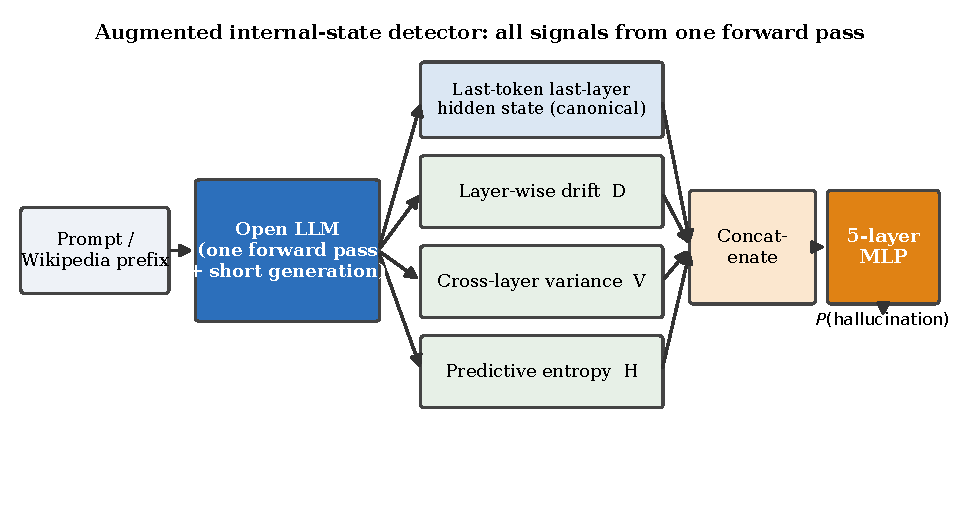
\includegraphics[width=0.99\textwidth]{images/ch04_methods/ch04_1_pipeline.pdf}
\caption{The augmented internal-state detector. Every signal is read from one forward
pass of a frozen model, so detection adds negligible cost over normal generation.}
\label{fig:pipeline}
\end{figure}

\section{Automatic label generation}
\label{sec:labels}

Supervised detection needs labelled examples, and labelling generations by hand does not
scale. We adopt the label-free procedure of the MIND framework~\cite{su2024mind},
illustrated in Figure~\ref{fig:pseudolabel} and stated as Algorithm~\ref{alg:label}. We
take an article, keep its first sentences, and find a named entity that occurs after the
first sentence. We truncate the text just before that entity and let the model predict
the continuation. If the entity the article actually had is among the model's top few
predicted first tokens, the model has stayed faithful, and we label the continuation
$y=0$. If the model instead produces a different entity, the continuation is factually
wrong with respect to the article; we let it generate on, then splice the article's
original suffix back so that the faithful and hallucinated versions differ only in the
entity span, and we label it $y=1$. The threshold for ``among the top few'' is the top
four predictions throughout.

\begin{figure}[h]
\centering
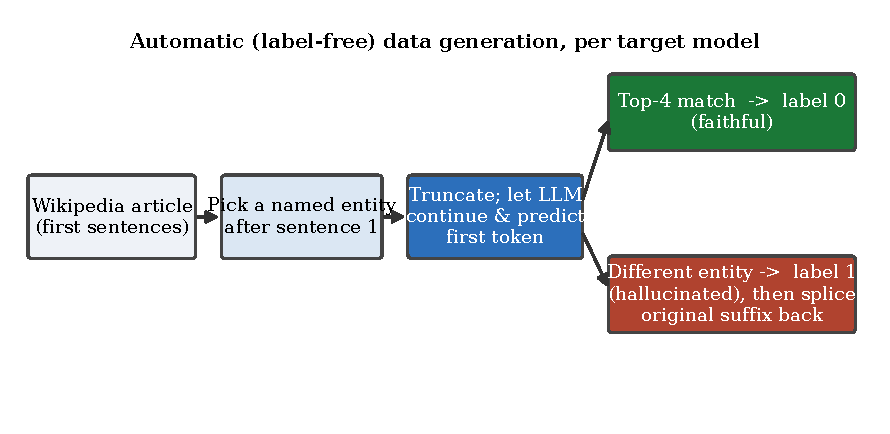
\includegraphics[width=0.96\textwidth]{images/ch04_methods/ch04_0_pseudolabel.pdf}
\caption{Automatic, label-free data generation. The model's own first-token prediction
decides the label; no human annotation is used, and the procedure is re-run separately
for each target model.}
\label{fig:pseudolabel}
\end{figure}

\begin{algorithm}[h]
\caption{Automatic label generation for one article}
\label{alg:label}
\begin{algbody}
\albf{Input:} article text, target model $M$, top-$k$ threshold $k=4$\\
\aln{1:}keep the first sentences; find a named entity $e$ occurring after sentence one\\
\aln{2:}truncate the text just before $e$ to form a prefix $x$\\
\aln{3:}let $M$ predict the next-token distribution given $x$\\
\aln{4:}\albf{if} $e$'s first token is among $M$'s top-$k$ predictions \albf{then}\\
\aln{5:}\alin label the continuation faithful ($y \gets 0$)\\
\aln{6:}\albf{else}\\
\aln{7:}\alin let $M$ generate until the original post-entity anchor reappears\\
\aln{8:}\alin splice the article's original suffix back onto the generated span\\
\aln{9:}\alin label the continuation hallucinated ($y \gets 1$)\\
\aln{10:}\albf{end if}\\
\aln{11:}\albf{return} labelled example $(x \,\Vert\, \text{continuation},\; y)$
\end{algbody}
\end{algorithm}

Two properties of this procedure matter. It produces balanced, per-model data at no
annotation cost, and --- because the prior literature shows probes do not transfer between
models --- it is run \emph{separately for each model} we study, so the training data always
comes from the same model the detector will monitor. For the larger models we generate one
thousand examples per class, two thousand in total.

\section{The canonical feature}

The backbone feature, which we call the \emph{canonical feature}, is the contextualised
vector at the last token of the final transformer layer~\cite{su2024mind}. Writing
$\zvec_\ell$ for the last-token activation at layer $\ell$ and $L$ for the number of
layers, the canonical feature is simply $\hvec = \zvec_L$. Its dimension equals the
model's hidden width $d$ --- for the six-billion-parameter model that anchors our results,
$d=4096$. Every configuration in the ablation includes this feature; the question the
ablation answers is what, if anything, the additional scalars buy on top of it.

\section{Three internal-state features}
\label{sec:trio}

The core proposal of this dissertation is to summarise the model's internal behaviour
during a generation with three inexpensive scalars, all computed from activations that
the forward pass already produced. We use fresh notation throughout: $\zvec_\ell$ is the
last-token activation vector at layer $\ell$, and $p_t(\cdot)$ is the model's token
distribution at generation step $t$.

\paragraph{Layer-wise representation drift.}
As information moves up the layer stack, the representation of a token changes. We measure
how much by the cosine distance between adjacent layers,
\begin{equation}
d_\ell \;=\; 1 - \frac{\zvec_\ell \cdot \zvec_{\ell+1}}{\lVert \zvec_\ell\rVert\,\lVert \zvec_{\ell+1}\rVert},
\qquad \ell = 1,\dots,L-1,
\end{equation}
and summarise the whole trajectory by its mean,
\begin{equation}
\Dmean \;=\; \frac{1}{L-1}\sum_{\ell=1}^{L-1} d_\ell .
\end{equation}
A faithful continuation tends to settle into a stable trajectory; large or erratic drift
is a candidate signal of trouble.

\paragraph{Cross-layer variance.}
A complementary view asks how spread out the layer representations are around their own
average. With the layer-wise mean $\bar{\zvec} = \tfrac{1}{L}\sum_{\ell=1}^{L}\zvec_\ell$,
we define
\begin{equation}
\Vlast \;=\; \frac{1}{L}\sum_{\ell=1}^{L}\bigl\lVert \zvec_\ell - \bar{\zvec}\bigr\rVert_2^{2}.
\end{equation}
Whereas drift is a sequential, layer-to-layer quantity, the variance is a global measure
of dispersion across the whole stack. Only the scalar $\Vlast$ is stored; the mean
$\bar{\zvec}$ is internal to its computation.

\paragraph{Predictive entropy.}
The third scalar looks at the output distribution rather than the hidden states. At each
generation step the Shannon entropy of the token distribution is
\begin{equation}
H^{(t)} \;=\; -\sum_{w \in V} p_t(w)\,\log p_t(w),
\end{equation}
where $V$ is the vocabulary, and we average it over the $T$ generated steps,
\begin{equation}
\Hmean \;=\; \frac{1}{T}\sum_{t=1}^{T} H^{(t)} .
\end{equation}
High predictive entropy means the model was unsure as it generated, which is weak but
useful evidence of hallucination.

The three scalars $\{\Dmean,\Vlast,\Hmean\}$ are concatenated onto the canonical feature.
Crucially, all three are intra-sample summaries from a single pass: they involve no extra
sampling, no auxiliary model, and no optimal-transport computation, which keeps them
clearly distinct from the prior study discussed in Section~\ref{sec:internal} and keeps
their cost negligible.

\section{Two wider feature families}

To place the three core features in context, the ablation also includes two further
families of scalar features, all read from the same single pass.

\paragraph{Literature features.}
A set of nine scalars is drawn from recent internal-state work. They include a
\emph{lookback ratio} that compares attention paid to the context against attention paid
to freshly generated tokens~\cite{chuang2024lookback}; an \emph{attention-sink} score
that measures how much attention mass collapses onto the first
token~\cite{xiao2023streamingllm}; a lightweight eigenvalue-based dispersion of the hidden
states in the spirit of the INSIDE method~\cite{chen2024inside}; an internal-consistency
ratio; a \emph{logit-lens divergence}, the Jensen--Shannon divergence (abbreviated JSD: a
symmetric measure of how different two probability distributions are) between the
vocabulary distributions read off from an early and a late layer, following the
contrast-between-layers idea~\cite{chuang2024dola}; an attention-head entropy; a
token-level confidence margin in the spirit of adaptive token-selection
work~\cite{niu2025hami}; the rank of the chosen token in the output distribution; and a
within-layer dispersion of token embeddings in the spirit of reasoning-aware
detection~\cite{d2hscore2025}. A tenth, supervised mid-layer probe feature is left for
future work because it would require training a separate probe inside the pipeline; we
note its omission rather than quietly dropping it.

\paragraph{Exploratory features.}
A second set of six scalars is more speculative and is included to test whether less
conventional signals help. In reader-facing terms these are: a small projection of the
hidden state through the model's output vocabulary head; a measure of the curvature of the
layer trajectory; the slope and variance of the model's confidence over the course of the
generation; an effective rank of the attention matrix; an alignment score between the
generated text and the prompt; and a divergence of the per-head importance distribution.
These are reported for completeness; we do not lean on them for any central claim.

\section{Feature configurations}
\label{sec:configs}

The ablation evaluates sixteen configurations, each being the canonical feature plus a
chosen subset of scalar features, as laid out in Figure~\ref{fig:families} and
Table~\ref{tab:configs}. The configurations move from the canonical feature alone, through
each new scalar added singly, to the three-scalar internal-state set, to the literature
set, to the exploratory set, and finally to combinations of these. Throughout the
dissertation we refer to configurations by a neutral index and a short description; we do
not use the working code names from the implementation. The configuration consisting of
the canonical feature plus the three internal-state scalars (configuration~5) is the
headline proposal, and we call it the \emph{augmented internal-state detector}.

\begin{figure}[t]
\centering
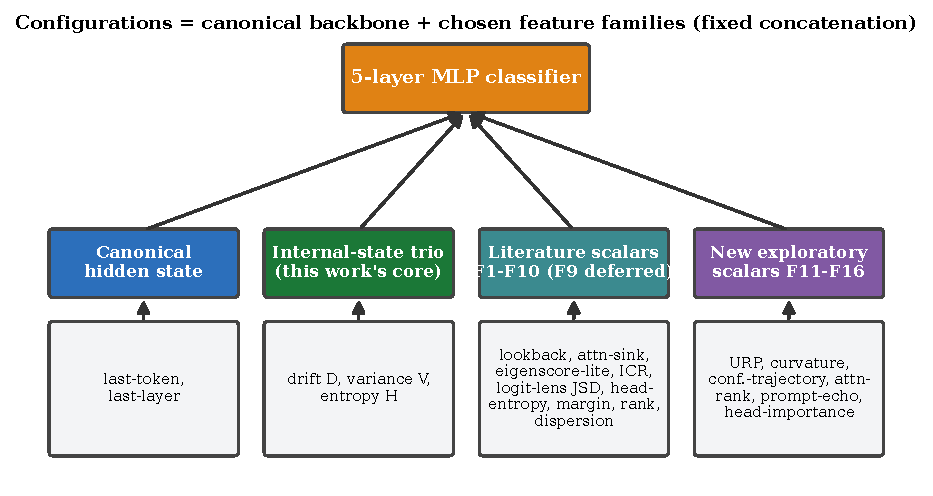
\includegraphics[width=0.97\textwidth]{images/ch04_methods/ch04_2_feature_families.pdf}
\caption{The feature families that make up the configurations. Each configuration is the
canonical backbone plus a fixed concatenation of chosen scalar families; there is no
automatic feature selection.}
\label{fig:families}
\end{figure}

\begin{table}[t]
\centering
\caption{The sixteen feature configurations. The input dimension is shown for the
six-billion-parameter model (hidden width $d=4096$); for other models the canonical part
changes with $d$ while the scalar counts stay the same.}
\label{tab:configs}
\small
\renewcommand{\arraystretch}{1.15}
\begin{tabular}{cl c c}
\toprule
\textbf{Cfg.} & \textbf{Feature content} & \textbf{\# scalars} & \textbf{MLP input dim} \\
\midrule
C1  & Canonical feature only (backbone)                         & 0  & 4096 \\
C2  & Canonical + drift                                         & 1  & 4097 \\
C3  & Canonical + cross-layer variance                          & 1  & 4097 \\
C4  & Canonical + predictive entropy                            & 1  & 4097 \\
C5  & Canonical + internal-state trio (\emph{this work})        & 3  & 4099 \\
C6  & Canonical + lookback ratio                                & 1  & 4097 \\
C7  & Canonical + logit-lens divergence                         & 1  & 4097 \\
C8  & Canonical + confidence margin                             & 1  & 4097 \\
C9  & Canonical + lookback/lens/margin trio                     & 3  & 4099 \\
C10 & Canonical + all nine literature features                  & 9  & 4105 \\
C11 & Canonical + internal-state trio + lookback/lens/margin     & 6  & 4102 \\
C12 & Canonical + internal-state trio + all literature           & 12 & 4108 \\
C13 & Canonical + vocab projection + curvature                  & 10 & 4106 \\
C14 & Canonical + confidence-trajectory/rank/echo               & 4  & 4100 \\
C15 & Canonical + vocab projection/curvature/confidence         & 12 & 4108 \\
C16 & Canonical + internal-state trio + all exploratory          & 18 & 4114 \\
\bottomrule
\end{tabular}
\end{table}

\section{The classifier}

Every configuration uses the same classifier, so that differences in measured performance
come from the features and not from the model on top of them. The classifier is a
five-layer perceptron with progressively narrowing hidden widths and rectified-linear
activations, ending in a two-way softmax that outputs the probability of each class. It is
trained with the cross-entropy loss using the Adam optimiser at a learning rate of
$5\times10^{-4}$ and weight decay $10^{-5}$, with a batch size of $32$, for ten epochs.
The scalar and canonical features are standardised by a scaler fitted on the training
split only, and the data is split $80/20$ into training and test sets with a fixed random
seed of $42$ so that every configuration sees exactly the same partition. The use of a
fixed, five-layer perceptron with cross-entropy and no feature selection is a deliberate
design commitment that distinguishes this work from the multi-feature, metric-learning
prior study of Section~\ref{sec:internal}.

\section{Evaluation protocol}
\label{sec:protocol}

After training on the encyclopedia-continuation data, each detector is evaluated in two
regimes. The \emph{in-distribution} regime uses a held-out split of the same
encyclopedia-continuation data. The \emph{transfer} regime uses a multi-benchmark suite
of question-answering, summarisation, and dialogue tasks that the detector never saw
during training. Algorithm~\ref{alg:eval} states the protocol.

To make the comparison fair and cheap, every method --- configuration or baseline --- is
scored on the \emph{same} fixed set of rows from each benchmark: a deterministic first-$N$
slice, with $N$ up to $350$ rows per benchmark in the fully unified runs. Because both the
configuration runs and the baseline runs read the same rows, their scores are directly
comparable. The transfer suite contains up to ten benchmarks: the four
question-answering sets TruthfulQA~\cite{lin2022truthfulqa},
TriviaQA~\cite{joshi2017triviaqa}, CoQA~\cite{reddy2019coqa} and
TyDi~QA~\cite{clark2020tydiqa}; the three directly labelled HaluEval
subsets~\cite{li2023halueval}; and three further question-answering sets, Natural
Questions~\cite{kwiatkowski2019nq}, HotpotQA~\cite{yang2018hotpotqa} and
PopQA~\cite{mallen2023popqa}. Each benchmark is wrapped in a short, fixed instruction
prompt appropriate to its task; the prompt wording is held constant across all methods.

\begin{algorithm}[h]
\caption{Single-pass feature extraction and multi-task evaluation}
\label{alg:eval}
\begin{algbody}
\albf{Input:} trained classifier $C$, target model $M$, benchmark suite $\mathcal{D}$, slice size $N$\\
\aln{1:}\albf{for} each benchmark $D \in \mathcal{D}$ \albf{do}\\
\aln{2:}\alin \albf{for} each of the first $N$ rows of $D$ \albf{do}\\
\aln{3:}\alinn run $M$ once on the prompt; collect last-layer hidden state and per-layer activations\\
\aln{4:}\alinn compute the canonical feature and the chosen scalars (drift, variance, entropy, \dots)\\
\aln{5:}\alinn standardise with the training scaler; obtain $\hat{p}=C(\mathbf{x})$\\
\aln{6:}\alin \albf{end for}\\
\aln{7:}\alin compute AUROC, accuracy, precision, recall, F1 (and calibration where available)\\
\aln{8:}\albf{end for}\\
\aln{9:}\albf{return} per-benchmark metrics and their mean
\end{algbody}
\end{algorithm}

\section{Baselines}
\label{sec:baselines}

The detectors are compared against four established methods plus two simple reference
methods, all re-implemented inside the same pipeline and scored on the same rows.
Table~\ref{tab:baselines} summarises them. SAPLMA~\cite{azaria2023saplma} is a supervised
probe on a single intermediate layer's hidden state. HaloScope~\cite{du2024haloscope} is
the unsupervised spectral method that estimates pseudo-labels from a latent subspace.
HalluShift~\cite{dasgupta2025hallushift} is the multi-feature supervised method of
Section~\ref{sec:internal}, re-implemented from its description with a thirty-one
dimensional feature vector. EigenScore is the sampling-based covariance score from the
INSIDE method~\cite{chen2024inside}. To these we add two reference points: MIND, a
supervised probe on the final-layer hidden state --- effectively the method this work
extends~\cite{su2024mind} --- and Perplexity, an unsupervised score equal to the mean
token negative log-likelihood (abbreviated NLL), where a higher value of the continuation's
perplexity is taken as weak evidence of hallucination.

Two further methods were considered as baselines and deliberately left out of the final
set. Semantic entropy~\cite{kuhn2023semantic} requires drawing several samples per prompt
and loading an auxiliary natural-language-inference model, which adds several hours of
computation per large model and would have broken the free-tier time budget. The
attention-only Lookback Lens~\cite{chuang2024lookback} was dropped because the attention
statistics it relies on are already represented among our features and among HalluShift's,
so it added a row without adding a new paradigm. The final baseline set is therefore the
four established methods plus the two reference scores.

\begin{table}[t]
\centering
\caption{Baselines re-implemented inside the unified pipeline. ``Dim'' is the
dimensionality of each method's feature or score for the six-billion-parameter model.}
\label{tab:baselines}
\small
\renewcommand{\arraystretch}{1.2}
\begin{tabularx}{\textwidth}{l l c X}
\toprule
\textbf{Baseline} & \textbf{Paradigm} & \textbf{Dim} & \textbf{Signal} \\
\midrule
SAPLMA      & supervised probe          & 4096 & hidden state at a single intermediate layer \\
HaloScope   & unsupervised spectral     & 4096 & best-layer hidden, pseudo-labelled from a subspace \\
HalluShift  & supervised multi-feature  & 31   & layer distribution-shift + attention + probability features \\
EigenScore  & sampling-based (score)    & 1    & log-determinant of the covariance of several samples \\
MIND        & supervised probe          & 4096 & final-layer last-token hidden state \\
Perplexity  & unsupervised (score)      & 1    & mean token negative log-likelihood \\
\bottomrule
\end{tabularx}
\end{table}

\section{Models and free-hardware implementation}
\label{sec:models}

A goal of this dissertation is that every experiment runs on free cloud hardware, so that
the study can be reproduced without a research budget. The primary platform is a free
Kaggle notebook with two T4 GPUs of sixteen gigabytes each, giving thirty-two gigabytes of
combined video memory (abbreviated VRAM) through model parallelism, used in the bfloat16
sixteen-bit number format (abbreviated bf16) with no further quantisation. Sessions are
capped at nine hours, within a weekly budget of thirty GPU-hours. A free Colab notebook
with a single T4 serves as a fallback for the smaller models. The seven-billion-parameter
models require both T4 GPUs; a single sixteen-gigabyte card cannot hold a seven-billion
model in bf16 together with the memory needed for generation.

Table~\ref{tab:models} lists the models. The fleet spans a tiny diagnostic model used only
to verify pipeline correctness, two sub-one-billion and one-to-three-billion models for
fast iteration, and a set of six- to seven-billion models that constitute the substantive
study. The six-billion-parameter model is the one for which a complete set of
configuration and baseline measurements exists, and it anchors the results of
Chapter~\ref{ch:results}.

\begin{table}[t]
\centering
\caption{Models in the study. ``Role'' distinguishes the substantive models from the small
models used for iteration and the tiny model used only as a correctness check. Hidden
width and layer count are listed where they anchor later results.}
\label{tab:models}
\small
\renewcommand{\arraystretch}{1.2}
\begin{tabular}{l c c l}
\toprule
\textbf{Model} & \textbf{Parameters} & \textbf{Hidden / layers} & \textbf{Role} \\
\midrule
GPT-J~\cite{wang2021gptj}            & 6.0\,B  & 4096 / 28 & substantive (complete measurements) \\
OPT~\cite{zhang2022opt}              & 6.7\,B  & 4096 / 32 & substantive \\
Llama-2~\cite{touvron2023llama2}     & 7\,B    & ---        & substantive (gated; data limited) \\
Mistral~\cite{jiang2023mistral}      & 7\,B    & ---        & substantive (results pending) \\
Falcon~\cite{almazrouei2023falcon}   & 7\,B    & ---        & substantive (results pending) \\
Qwen2.5~\cite{qwen2024report}        & 3\,B    & 2560 / --- & iteration / in-distribution \\
TinyLlama~\cite{zhang2024tinyllama}  & 1.1\,B  & 2048 / --- & iteration / in-distribution \\
Qwen2.5 (small)~\cite{qwen2024report}& 0.5\,B  & ---        & fast iteration \\
GPT-2~\cite{radford2019gpt2}         & 0.12\,B & ---        & smoke test (diagnostic only) \\
\bottomrule
\end{tabular}
\end{table}

In summary, the methodology fixes everything except the features: the same automatic
labels, the same classifier, the same split and seed, the same evaluation rows, and the
same hardware regime. This is what makes the comparison in the next chapter a comparison
of \emph{features}, and what makes it reproducible on a free account.

% =====================================================================
\chapter{Results and Discussion}
\label{ch:results}
% =====================================================================

This chapter reports what the experiments actually show. We are deliberately strict about
provenance: a number appears here only if a saved measurement file supports it, and we
keep in-distribution detection separate from cross-task transfer at all times. The chapter
first states which experiments are complete and which are still running, then presents the
in-distribution results, then the full transfer results for the one model with a complete
set of measurements, then a partial second model, and finally the discussion.

\section{What has been measured}

The study spans several models, but they are at different stages of completion, and it
would be misleading to present them as a finished sweep. Table~\ref{tab:status} states the
status of each model honestly. One six-billion-parameter model has a complete set of
measurements --- all sixteen configurations and all six baselines, on all ten benchmarks,
scored on identical rows --- and it anchors this chapter. A second model of comparable size
has a verifiable diagnostic run plus an extended run whose consolidated file is not yet
archived. The remaining large models have generated their training data but do not yet
have reported detection results, and are marked accordingly.

\begin{table}[h]
\centering
\caption{Status of each model at the time of writing. Only the model with a complete,
file-backed set of measurements is used for the headline comparison.}
\label{tab:status}
\small
\renewcommand{\arraystretch}{1.2}
\begin{tabular}{l c l}
\toprule
\textbf{Model} & \textbf{Training examples} & \textbf{Status} \\
\midrule
GPT-J (6.0\,B)      & 2000 & complete: 16 configurations + 6 baselines, 10 benchmarks \\
OPT (6.7\,B)        & 2000 & partial: diagnostic run verified; extended run pending archival \\
Qwen2.5 (3\,B)      & 2000 & in-distribution configurations only (no baseline run) \\
TinyLlama (1.1\,B)  & ---  & earlier in-distribution figure only \\
Mistral (7\,B)      & 2000 & data generated; detection results pending \\
Falcon (7\,B)       & 2000 & data generated; detection results pending \\
Llama-2 (7\,B)      & 400  & gated access; undersized data; results pending \\
GPT-2 (0.12\,B)     & 1000 & smoke test; diagnostic only, not a result \\
\bottomrule
\end{tabular}
\end{table}

\section{In-distribution detection}

We begin with the easier regime, in which the detector is tested on held-out text of the
same kind it was trained on. An earlier mid-term evaluation, run on a larger
ten-thousand-sample corpus with the canonical feature alone, reported in-distribution
AUROC of $0.673$ for the three-billion model and $0.592$ for the one-billion model, and
noted that the larger model carried the stronger internal signal. These are encouraging
numbers, but they are in-distribution and were obtained at a larger data scale than the
unified runs reported below.

At the two-thousand-sample scale of the unified pipeline, in-distribution AUROC is more
modest. On the three-billion model the configurations sit between roughly $0.39$ and
$0.47$, and on the six-billion model they sit between roughly $0.40$ and $0.55$. The drop
relative to the mid-term figure is consistent with the smaller training set and the harder,
fully unified evaluation; it is a reminder that sample size matters and that a single
favourable number should not be over-read. Figure~\ref{fig:indist} places the in-distribution
and transfer numbers side by side and makes the central point of this chapter visible at a
glance: in-distribution detection, while imperfect, is clearly easier than transferring to
unseen task types.

\begin{figure}[t]
\centering
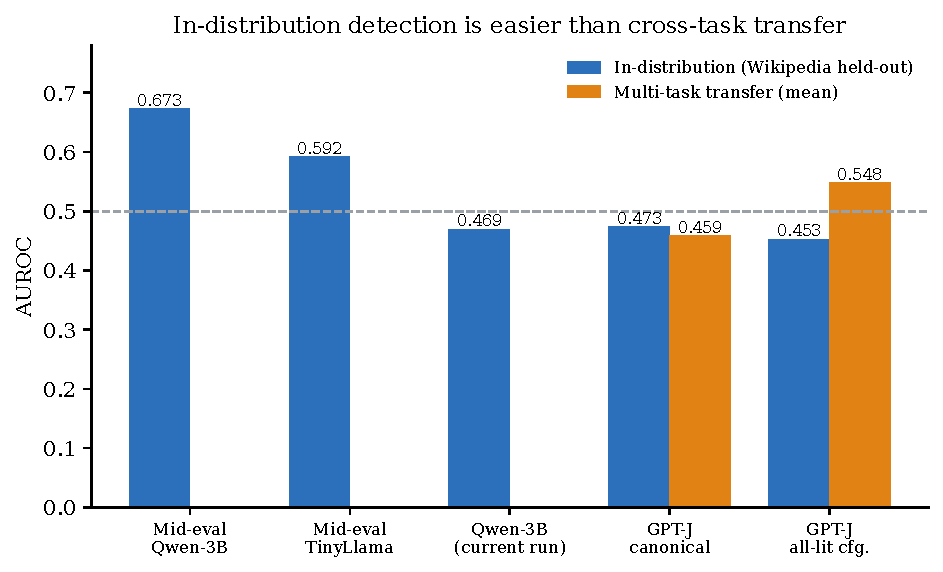
\includegraphics[width=0.84\textwidth]{images/ch05_results/ch05_4_indist_vs_transfer.pdf}
\caption{In-distribution detection is easier than cross-task transfer. The two left bars
are earlier mid-term in-distribution figures at a larger data scale; the rest are from the
unified runs. Transfer means are computed over the ten-benchmark suite.}
\label{fig:indist}
\end{figure}

\section{Transfer results on the fully measured model}
\label{sec:gptj}

We now turn to the substantive result: cross-task transfer on the six-billion-parameter
model, for which every configuration and baseline was measured on the same rows of all ten
benchmarks. Table~\ref{tab:gptj-configs} reports the sixteen configurations and
Table~\ref{tab:gptj-base} the six baselines, each by mean transfer AUROC; the full
per-benchmark matrix is given in Appendix~\ref{app:tables}.

\begin{table}[h]
\centering
\caption{Six-billion-parameter model: the sixteen feature configurations, by mean transfer
AUROC over ten benchmarks, with the in-distribution figure for reference. Higher is
better; $0.5$ is chance.}
\label{tab:gptj-configs}
\small
\renewcommand{\arraystretch}{1.15}
\begin{tabular}{cl c c}
\toprule
\textbf{Cfg.} & \textbf{Feature content} & \textbf{In-distribution} & \textbf{Mean transfer} \\
\midrule
C1  & Canonical feature only                       & 0.473 & 0.459 \\
C2  & + drift                                      & 0.500 & 0.447 \\
C3  & + cross-layer variance                       & 0.525 & 0.445 \\
C4  & + predictive entropy                         & 0.404 & 0.472 \\
C5  & + internal-state trio (\emph{this work})     & 0.500 & 0.464 \\
C6  & + lookback ratio                             & 0.524 & 0.445 \\
C7  & + logit-lens divergence                      & 0.498 & 0.446 \\
C8  & + confidence margin                          & 0.546 & 0.476 \\
C9  & + lookback/lens/margin trio                  & 0.481 & 0.446 \\
C10 & + all nine literature features               & 0.453 & \textbf{0.548} \\
C11 & + internal-state trio + lookback/lens/margin & 0.540 & 0.525 \\
C12 & + internal-state trio + all literature       & 0.475 & 0.468 \\
C13 & + vocab projection + curvature               & 0.488 & 0.451 \\
C14 & + confidence-trajectory/rank/echo            & 0.405 & 0.546 \\
C15 & + vocab projection/curvature/confidence      & 0.508 & 0.471 \\
C16 & + internal-state trio + all exploratory      & 0.507 & 0.508 \\
\bottomrule
\end{tabular}
\end{table}

\begin{table}[h]
\centering
\caption{Six-billion-parameter model: the six baselines, by mean transfer AUROC over ten
benchmarks. The strongest method overall is the supervised mid-layer probe.}
\label{tab:gptj-base}
\small
\renewcommand{\arraystretch}{1.2}
\begin{tabular}{l c c}
\toprule
\textbf{Baseline} & \textbf{In-distribution} & \textbf{Mean transfer} \\
\midrule
SAPLMA (mid-layer probe)   & 0.419 & \textbf{0.562} \\
Perplexity (mean NLL)      & ---   & 0.523 \\
HalluShift                 & 0.519 & 0.509 \\
HaloScope                  & 0.506 & 0.508 \\
MIND (final-layer probe)   & ---   & 0.487 \\
EigenScore                 & 0.515 & 0.487 \\
\bottomrule
\end{tabular}
\end{table}

The picture that emerges is mixed, and we report it as such. Ranked by mean transfer
AUROC, the strongest method is the supervised mid-layer probe, SAPLMA, at $0.562$. The two
best feature configurations follow closely: the all-literature configuration at $0.548$
and the confidence-trajectory configuration at $0.546$, with the configuration that adds
the internal-state trio to a small literature subset close behind at $0.525$. The simple
perplexity reference scores $0.523$, ahead of the more elaborate HalluShift, HaloScope,
final-layer MIND, and EigenScore baselines, all of which sit between $0.487$ and $0.509$.
Figure~\ref{fig:configs} and Figure~\ref{fig:methods} show these comparisons graphically.

\begin{figure}[t]
\centering
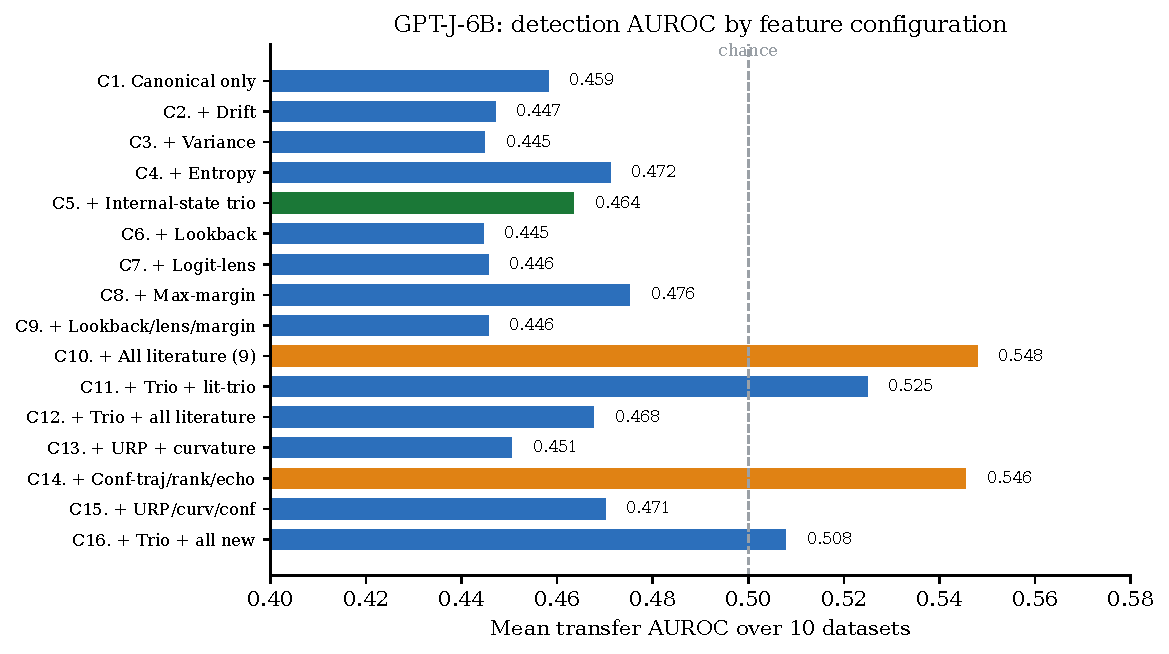
\includegraphics[width=0.95\textwidth]{images/ch05_results/ch05_1_gptj_config_auroc.pdf}
\caption{Mean transfer AUROC of the sixteen configurations on the six-billion model. The
three-feature internal-state set (highlighted) gives only a small change over the
canonical backbone; the gains come from the richer stacks (highlighted).}
\label{fig:configs}
\end{figure}

\begin{figure}[t]
\centering
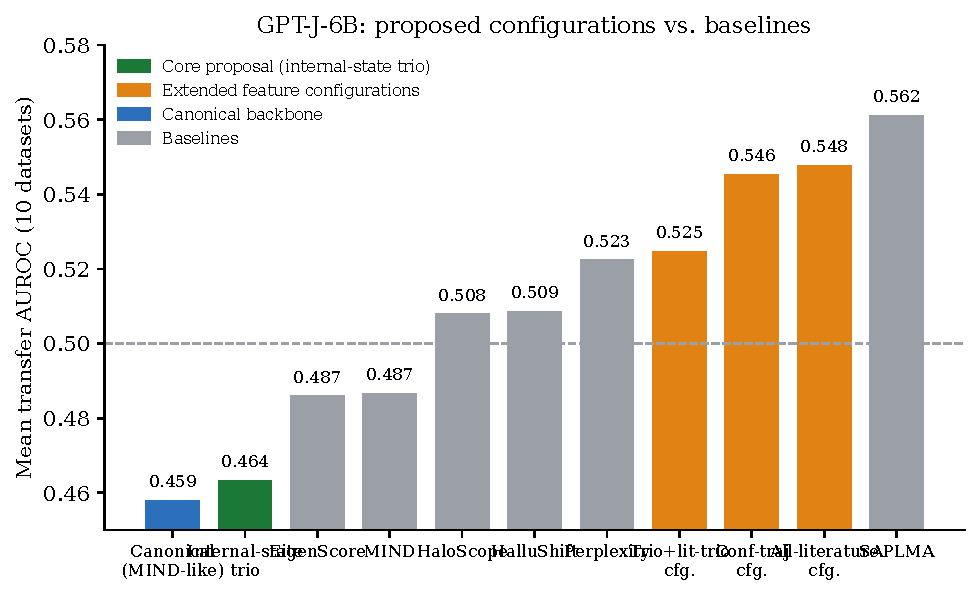
\includegraphics[width=0.95\textwidth]{images/ch05_results/ch05_2_gptj_method_vs_baselines.pdf}
\caption{The proposed configurations against the baselines on the six-billion model. The
best configurations are competitive with the field but do not overtake the strongest
baseline, the supervised mid-layer probe.}
\label{fig:methods}
\end{figure}

Three observations follow directly from these numbers. First, the three core
internal-state features, taken alone on top of the canonical feature (configuration~5),
move the mean transfer AUROC only slightly, from $0.459$ to $0.464$; the individual
additions are mixed, with predictive entropy and the confidence margin helping a little
and drift or variance alone not helping. The lift that does appear comes from the richer
combinations of many features at once. Second, the strongest baseline reads a
\emph{mid-network} layer, while the canonical feature and the MIND baseline read the
\emph{final} layer, and the mid-layer probe is clearly better here ($0.562$ versus
$0.487$). This echoes the layer-selection problem flagged in the literature: on this
model the last layer is not the most informative place to look. Third, none of the
methods is far above chance on transfer; the averages sit in the high-$0.4$ to
mid-$0.5$ range, which is honest evidence that transferring an encyclopedia-trained probe
to unseen task types is hard.

\section{One benchmark dominates the averages}

Before reading too much into the rankings, it is important to see how they are formed.
Figure~\ref{fig:heatmap} shows the per-benchmark AUROC for a representative set of methods,
and Figure~\ref{fig:dominance} traces the same numbers as lines. One benchmark, the
question-answering subset of HaluEval, behaves very differently from the rest: the
mid-layer probe reaches $0.985$ on it, the confidence-trajectory configuration $0.94$, and
the all-literature configuration $0.84$, while on the other nine benchmarks almost every
method hovers near $0.5$. Because this one column is so high, it pulls the averages up and
largely determines the ranking. The honest reading is that the headline averages are
carried by a single, unusually separable benchmark, and that on the remaining benchmarks
the methods are much closer together and much closer to chance. A ranking that looks
decisive on paper is, on inspection, the product of one easy column.

\begin{figure}[t]
\centering
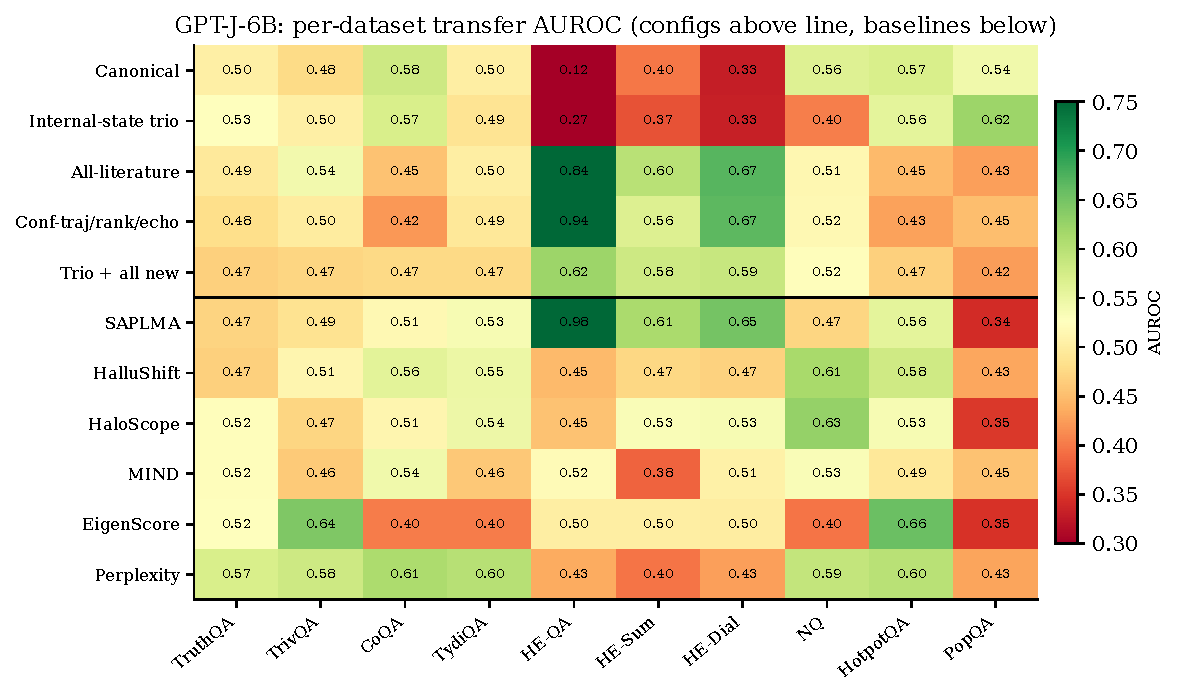
\includegraphics[width=0.99\textwidth]{images/ch05_results/ch05_3_gptj_heatmap.pdf}
\caption{Per-benchmark transfer AUROC on the six-billion model, configurations above the
line and baselines below. The HaluEval-QA column stands out; elsewhere most cells are near
$0.5$.}
\label{fig:heatmap}
\end{figure}

\begin{figure}[t]
\centering
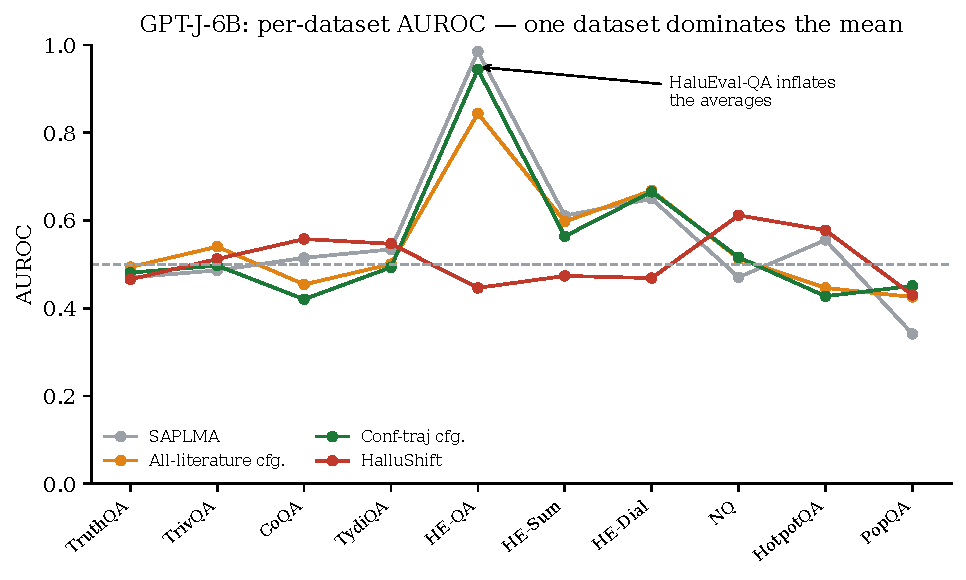
\includegraphics[width=0.86\textwidth]{images/ch05_results/ch05_5_halueval_dominance.pdf}
\caption{The same data as lines. The spike on HaluEval-QA is what separates the leading
methods; the other benchmarks cluster near chance.}
\label{fig:dominance}
\end{figure}

\section{A partial second model}

The second six-billion-class model gives a complementary, but only partly verifiable,
picture. The configuration run whose measurement file is present in the repository covers
the original seven-benchmark suite at a small number of rows per benchmark; on it, every
configuration sits near or below chance on average (the best, the all-literature
configuration, averages about $0.44$ over the seven benchmarks), which at that small
sample size is best read as diagnostic rather than scientific. An extended run on the full
ten-benchmark suite with the four established baselines is recorded in the project's
comparison table, and in it the confidence-trajectory configuration leads on average,
ahead of the mid-layer probe and HalluShift. We report this extended result as
\emph{indicative}: its consolidated measurement file is not part of the current repository
snapshot, so by the provenance rule of this chapter we do not treat its numbers as
verified, and we will update them when the file is archived. What can be said responsibly
is that the two models disagree about which method leads --- a supervised baseline on one,
a proposed feature configuration on the other --- which is itself the finding.

\section{Models still in progress}

Three further seven-billion models have completed the data-generation stage but do not yet
have reported detection results, and are listed as pending in Table~\ref{tab:status}. One
of them is gated and currently has an undersized training set, which must be regenerated
before its numbers will be comparable. The tiny diagnostic model behaves exactly as
expected for its scale: its AUROCs scatter around chance and its classifier frequently
collapses to a single class on the small test set. We use it only to confirm that the
pipeline is correct end to end, and we do not present its numbers as findings.

\section{Discussion}

Taken together, the results support a measured set of conclusions rather than a triumphant
one.

The internal-state signal is real but, on transfer, weak. In-distribution detection works
at a useful level, especially at larger data scales, but transferring a probe trained on
encyclopedia continuations to question answering, summarisation, and dialogue is hard, and
all methods --- ours and the baselines --- struggle once the one easy benchmark is set aside.
This is not a defect of any single method; it is a property of the task, and it is the most
important thing the experiments show.

The three core features proposed here are inexpensive and well motivated, but on the fully
measured model they add little on their own. Where the proposed work is competitive is in
the richer configurations, and even there it matches rather than beats the strongest
baseline. The strongest baseline's advantage appears to come less from a clever feature
than from reading a better layer, which points to layer selection --- not feature count ---
as the lever most worth pulling next.

The comparison is model-dependent. On the fully measured model a supervised baseline leads;
on the partially measured model an extended run favours a proposed configuration. With only
one fully verified model it would be wrong to generalise in either direction, and we do
not. This is exactly why the contribution of the dissertation is framed as a reproducible
comparison rather than a new state of the art: the value of the comparison is that it makes
these model-dependent, regime-dependent effects visible and checkable, on hardware anyone
can rent for free.

% =====================================================================
\chapter{Conclusion and Future Work}
\label{ch:conclusion}
% =====================================================================

\section{Summary}

This dissertation studied whether hallucinations in large language models can be detected
cheaply by reading the model's own internal representations, and which of the many proposed
internal signals are worth their cost. We adopted the label-free, per-model data generation
of the MIND framework, kept its canonical last-token, last-layer hidden state as a backbone,
and added three inexpensive signals from the same forward pass: how much the representation
drifts between layers, how much it varies across layers, and how uncertain the model is while
generating. We placed these in a controlled ablation alongside literature features and more
speculative features, fixed a single classifier and a single evaluation protocol, and
compared everything against four established baselines and two simple reference methods on a
suite of up to ten benchmarks --- all on free cloud hardware.

The honest summary of the findings is threefold. First, detection of held-out
in-distribution text works at a useful level, and better at larger data scales, but
transferring an encyclopedia-trained probe to question answering, summarisation, and dialogue
is hard: on transfer, every method we tested sits close to chance once a single unusually
separable benchmark is set aside. Second, on the one model for which we have a complete set
of file-backed measurements, the three core features add little on their own, the gains come
from richer feature combinations, and even the best configurations match rather than beat the
strongest baseline --- a supervised probe whose advantage seems to come from reading a better
layer rather than from a cleverer feature. Third, the result is model-dependent: on a second
model of comparable size a proposed configuration --- built from the more exploratory
internal-state signals --- is instead the strongest method of all, clearing every baseline.
Two models of similar size disagreeing about which method wins is itself the finding, and a
caution against reading a universal winner off any one model.

The contribution is therefore not a new state-of-the-art detector. It is a unified,
free-tier-reproducible comparison of internal-state hallucination features across several open
models, built so that the regime-dependent and model-dependent effects above are visible and
checkable rather than hidden inside a single headline number.

\section{Limitations}

We state the limitations plainly, because several of them bound how far the conclusions can
be taken.

\textbf{Two models, not the whole fleet.} The comparison rests on two six-billion-parameter
models: one with the complete sixteen-configuration, six-baseline sweep, and one with the six
baselines measured against the exploratory-feature configurations. The remaining large models
have their training data ready but their detection runs are still in progress, so the
cross-model claim is drawn from two models rather than the full fleet.

\textbf{Modest sample sizes.} The unified runs use two thousand training examples per model
and evaluate on a few hundred rows per benchmark. At this scale, individual AUROCs are noisy,
classifiers sometimes collapse to a single class, and small differences between methods should
not be over-interpreted. The earlier, larger-scale in-distribution figures suggest that more
data helps, but we did not re-run the full ablation at that scale.

\textbf{Free-tier constraints.} The nine-hour session limit, the weekly GPU budget, and the
sixteen-gigabyte cards shaped the design: some baselines were dropped for cost, evaluation was
capped at a fixed number of rows, and one gated model could not be run at full data size.
These are reasonable trade-offs for a reproducible free-hardware study, but they are
constraints, and a better-resourced replication might reach steadier numbers.

\textbf{One benchmark dominates.} The transfer averages on the fully measured model are
carried by a single easy benchmark. The rankings should be read with that in mind, and
per-benchmark results (Appendix~\ref{app:tables}) are more informative than the averages.

\textbf{Split evaluation on the second model.} On the second model the literature and
core-feature configurations were scored on the earlier seven-benchmark suite while the
exploratory-feature configurations and the baselines used the full ten; a single unified
re-run would put all sixteen configurations on the same footing.

\section{Future work}

Several concrete next steps follow from these limitations.

The most immediate is to \emph{complete the sweep}: run the full sixteen-configuration,
six-baseline comparison on the second model and on the remaining seven-billion models, and
regenerate the gated model's data at full size. This broadens a two-model comparison into a
fleet-wide one and would settle whether the model-dependence seen here is the rule.

The discussion pointed at \emph{layer selection} as the lever most worth pulling. The strongest
baseline's edge came from reading a mid-network layer rather than the final one, so a focused
ablation over the layer at which the canonical and internal-state features are read --- on each
model --- is likely to be more productive than adding further scalar features.

A third direction is \emph{scale and calibration}. Re-running the ablation at the larger
data scale used in the mid-term evaluation would test whether the small per-feature effects
become reliable, and reporting calibration error and Brier score alongside AUROC would make the
detectors more useful as decision-support tools, since a calibrated probability is worth more
than a bare verdict.

Finally, the finding that transfer is the hard part suggests studying the \emph{training
distribution} itself: mixing a small amount of task-like data into the encyclopedia
continuations, or generating continuations from more varied sources, may close part of the
in-distribution-to-transfer gap that dominates the present results.

\section{Closing remark}

The modest headline of this work --- that inexpensive internal-state features are competitive
but not decisive, and that cross-task transfer remains hard --- is, we think, more useful than a
louder claim would have been. The detectors in this area are often reported under favourable,
inconsistent conditions; holding everything fixed and running them on free hardware shows where
the real difficulty lies. Making that difficulty visible, and reproducible, is the point.

\clearpage
\addcontentsline{toc}{chapter}{References}
\bibliographystyle{unsrt}
\bibliography{references}
\appendix
% =====================================================================
\chapter{Full Result Tables}
\label{app:tables}
% =====================================================================

This appendix gives the complete per-benchmark measurements behind the summary figures and
tables of Chapter~\ref{ch:results}. All numbers are AUROC, read directly from the saved
measurement files; $0.5$ is chance.

Table~\ref{tab:app-gptj-full} is the full matrix for the six-billion-parameter model that
anchors the study: every one of the sixteen configurations and six baselines, scored on the
same rows of all ten benchmarks. It is the table from which the means in
Section~\ref{sec:gptj} are computed, and it makes the per-benchmark spread --- in particular
the dominance of the HaluEval-QA column --- explicit.

\begin{table}[h]
\centering
\caption{Full per-benchmark transfer AUROC on the six-billion-parameter model (GPT-J): sixteen feature configurations and six baselines, scored on identical rows of all ten benchmarks. \textbf{Bold} marks the best value in each column. Source: the consolidated configuration and baseline measurement files.}
\label{tab:app-gptj-full}
\footnotesize
\setlength{\tabcolsep}{3.2pt}
\begin{tabular}{lcccccccccc|c}
\toprule
Method & TruthQA & TrivQA & CoQA & TydiQA & HE-QA & HE-Sm & HE-Dl & NQ & HotQA & PopQA & Avg \\
\midrule
C1 canonical & 0.503 & 0.476 & 0.580 & 0.502 & 0.124 & 0.398 & 0.330 & 0.562 & 0.569 & 0.541 & 0.459 \\
C2 {+}drift & 0.492 & 0.459 & 0.566 & 0.492 & 0.127 & 0.337 & 0.339 & 0.551 & 0.558 & 0.553 & 0.447 \\
C3 {+}variance & 0.478 & 0.453 & 0.564 & 0.497 & 0.109 & 0.381 & 0.349 & 0.535 & 0.554 & 0.534 & 0.445 \\
C4 {+}entropy & 0.519 & 0.410 & 0.541 & 0.478 & 0.260 & 0.389 & 0.389 & 0.513 & 0.524 & \textbf{0.692} & 0.472 \\
C5 {+}trio & 0.526 & 0.503 & 0.570 & 0.487 & 0.272 & 0.371 & 0.330 & 0.403 & 0.557 & 0.620 & 0.464 \\
C6 {+}lookback & 0.498 & 0.483 & 0.591 & 0.505 & 0.068 & 0.342 & 0.321 & 0.544 & 0.550 & 0.548 & 0.445 \\
C7 {+}logit-lens & 0.472 & 0.482 & 0.573 & 0.502 & 0.079 & 0.383 & 0.344 & 0.535 & 0.546 & 0.545 & 0.446 \\
C8 {+}margin & 0.522 & 0.478 & 0.525 & 0.536 & 0.434 & 0.374 & 0.396 & 0.558 & 0.517 & 0.417 & 0.476 \\
C9 {+}l/l/m & 0.504 & 0.511 & 0.563 & 0.490 & 0.126 & 0.348 & 0.329 & 0.455 & 0.563 & 0.569 & 0.446 \\
C10 {+}all lit. & 0.494 & 0.540 & 0.454 & 0.501 & 0.844 & 0.597 & \textbf{0.668} & 0.513 & 0.446 & 0.426 & 0.548 \\
C11 {+}trio{+}llm & 0.484 & 0.518 & 0.546 & 0.520 & 0.635 & 0.391 & 0.464 & 0.539 & 0.603 & 0.553 & 0.525 \\
C12 {+}trio{+}lit. & 0.555 & 0.534 & 0.444 & 0.465 & 0.408 & 0.462 & 0.522 & 0.484 & 0.453 & 0.355 & 0.468 \\
C13 {+}urp/curv & 0.494 & 0.507 & 0.576 & 0.507 & 0.065 & 0.315 & 0.311 & 0.572 & 0.567 & 0.596 & 0.451 \\
C14 {+}conf-traj & 0.481 & 0.497 & 0.421 & 0.493 & 0.944 & 0.564 & 0.665 & 0.516 & 0.427 & 0.451 & 0.546 \\
C15 {+}urp/cv/cf & 0.504 & 0.481 & 0.440 & 0.461 & 0.351 & 0.527 & 0.406 & 0.604 & 0.449 & 0.483 & 0.471 \\
C16 {+}trio{+}new & 0.465 & 0.471 & 0.475 & 0.475 & 0.620 & 0.580 & 0.585 & 0.522 & 0.466 & 0.424 & 0.508 \\
\midrule
\multicolumn{12}{l}{\emph{Baselines}}\\
SAPLMA & 0.470 & 0.486 & 0.515 & 0.534 & \textbf{0.985} & \textbf{0.611} & 0.649 & 0.471 & 0.555 & 0.341 & \textbf{0.562} \\
Perplexity & \textbf{0.570} & 0.580 & \textbf{0.609} & \textbf{0.600} & 0.434 & 0.397 & 0.426 & 0.589 & 0.597 & 0.429 & 0.523 \\
HalluShift & 0.466 & 0.512 & 0.558 & 0.547 & 0.446 & 0.474 & 0.469 & 0.612 & 0.578 & 0.430 & 0.509 \\
HaloScope & 0.523 & 0.472 & 0.512 & 0.545 & 0.455 & 0.531 & 0.535 & \textbf{0.627} & 0.534 & 0.352 & 0.508 \\
MIND & 0.522 & 0.462 & 0.542 & 0.458 & 0.520 & 0.384 & 0.505 & 0.532 & 0.493 & 0.453 & 0.487 \\
EigenScore & 0.523 & \textbf{0.641} & 0.400 & 0.402 & 0.501 & 0.500 & 0.500 & 0.395 & \textbf{0.656} & 0.347 & 0.487 \\
\bottomrule
\end{tabular}
\end{table}

Table~\ref{tab:app-opt-diag} is the file-backed diagnostic run for the second
six-billion-class model. It covers twelve configurations on the original seven-benchmark
suite at a small number of rows per benchmark; as noted in Chapter~\ref{ch:results}, these
numbers are diagnostic rather than scientific, and the extended ten-benchmark run with
baselines is awaiting archival.

\begin{table}[h]
\centering
\caption{Diagnostic configuration run on the second six-billion-class model (OPT-6.7B), the part backed by a measurement file in the repository: twelve configurations on the original seven-benchmark suite at a small number of rows per benchmark. At this sample size the numbers are diagnostic, not scientific. AUROC; $0.5$ is chance.}
\label{tab:app-opt-diag}
\footnotesize
\setlength{\tabcolsep}{4pt}
\begin{tabular}{lccccccc|c}
\toprule
Cfg. & TruthQA & TrivQA & CoQA & TydiQA & HE-QA & HE-Sm & HE-Dl & Avg \\
\midrule
C1 canonical & 0.328 & 0.535 & 0.571 & 0.503 & 0.054 & 0.423 & 0.345 & 0.394 \\
C2 {+}drift & 0.338 & 0.567 & 0.564 & 0.523 & 0.039 & 0.316 & 0.313 & 0.380 \\
C3 {+}variance & 0.308 & 0.561 & 0.550 & 0.537 & 0.025 & 0.321 & 0.310 & 0.373 \\
C4 {+}entropy & 0.303 & 0.539 & 0.556 & 0.542 & 0.126 & 0.342 & 0.336 & 0.392 \\
C5 {+}trio & 0.276 & 0.485 & 0.502 & 0.492 & 0.228 & 0.380 & 0.342 & 0.386 \\
C6 {+}lookback & 0.286 & 0.546 & 0.558 & 0.506 & 0.032 & 0.361 & 0.316 & 0.372 \\
C7 {+}logit-lens & 0.313 & 0.527 & 0.542 & 0.514 & 0.026 & 0.336 & 0.309 & 0.367 \\
C8 {+}margin & 0.308 & 0.528 & 0.559 & 0.516 & 0.037 & 0.335 & 0.313 & 0.371 \\
C9 {+}l/l/m & 0.303 & 0.519 & 0.551 & 0.504 & 0.055 & 0.334 & 0.349 & 0.374 \\
C10 {+}all lit. & 0.308 & 0.626 & 0.562 & 0.567 & 0.246 & 0.395 & 0.353 & 0.437 \\
C11 {+}trio{+}llm & 0.328 & 0.553 & 0.551 & 0.538 & 0.049 & 0.286 & 0.302 & 0.373 \\
C12 {+}trio{+}lit. & 0.293 & 0.528 & 0.554 & 0.498 & 0.020 & 0.352 & 0.318 & 0.366 \\
\bottomrule
\end{tabular}
\end{table}

% =====================================================================
\chapter{Hyperparameters and Implementation Details}
\label{app:hyper}
% =====================================================================

For reproducibility, this appendix records the settings used throughout. All runs use a
fixed random seed of $42$.

\section*{Data generation}
\begin{itemize}[leftmargin=1.6em,itemsep=0.2em]
\item Source text: encyclopedia articles; the first sentences are retained and a named
entity occurring after the first sentence is selected.
\item Faithful/hallucinated decision: the original entity's first token must appear among
the model's top four predicted tokens to be labelled faithful.
\item Generation cap during labelling: a short continuation of up to $48$ new tokens.
\item Scale: one thousand examples per class (two thousand total) for the large models;
smaller counts for the iteration and smoke models, as recorded in Chapter~\ref{ch:results}.
\item Numeric format: bfloat16, with no further quantisation.
\end{itemize}

\section*{Classifier}
\begin{itemize}[leftmargin=1.6em,itemsep=0.2em]
\item Architecture: a five-layer perceptron with progressively narrowing hidden widths,
rectified-linear activations, and a two-way softmax output.
\item Loss and optimiser: cross-entropy; Adam with learning rate $5\times10^{-4}$ and weight
decay $10^{-5}$.
\item Batch size $32$; ten training epochs.
\item Features standardised by a scaler fitted on the training split only.
\item Split: $80\%$ train / $20\%$ test, identical across all configurations.
\end{itemize}

\section*{Evaluation}
\begin{itemize}[leftmargin=1.6em,itemsep=0.2em]
\item Each method --- configuration or baseline --- is scored on the same deterministic
first-$N$ slice of each benchmark, with $N$ up to $350$ rows per benchmark in the unified
runs.
\item Metrics: AUROC (primary), accuracy, precision, recall, F1; calibration (Brier score,
expected calibration error) where the measurement file records it.
\item In-distribution and transfer numbers are never averaged together.
\end{itemize}

\section*{Baseline settings (six-billion model)}
\begin{itemize}[leftmargin=1.6em,itemsep=0.2em]
\item Supervised mid-layer probe: hidden state read at an intermediate layer (layer $17$ of
$28$).
\item Logit-lens divergence feature: early/late comparison taken at layer $14$.
\item Spectral baseline: best layer and threshold selected on a validation split.
\item Sampling-based score: a small number of stochastic samples per query, with a ridge
term for numerical stability.
\end{itemize}

\section*{Hardware}
\begin{itemize}[leftmargin=1.6em,itemsep=0.2em]
\item Primary: a free cloud notebook with two sixteen-gigabyte T4 GPUs (thirty-two gigabytes
combined), nine-hour session cap, thirty GPU-hours per week.
\item Fallback: a free single-T4 notebook for the smaller models.
\item The seven-billion models require both GPUs; a single sixteen-gigabyte card cannot hold
a seven-billion model in bfloat16 together with generation memory.
\end{itemize}

% =====================================================================
\chapter{Reproducibility Notes}
\label{app:repro}
% =====================================================================

The study is designed to be reproducible on a free account. Three points are worth
emphasising. First, the training data is generated separately for each model, because probes
do not transfer between models; a detector is therefore always trained on data from the same
model it monitors. Second, every configuration and baseline within a model shares the same
generated data, the same train/test split and seed, and the same evaluation rows, so that
differences in measured performance are attributable to the features rather than to incidental
differences in setup. Third, the evaluation benchmarks are downloaded once and cached so that
runs are not dependent on network conditions, and the per-benchmark row count is fixed so that
cost stays within the free-tier budget. Where a model's measurement file is not yet archived,
its numbers are marked as pending in Chapter~\ref{ch:results} rather than reported as results.

\end{document}
